% siminos/blog/PoincSecBlog.tex
% $Author: xiong $ $Date: 2017-04-14 23:39:47 -0400 (Fri, 14 Apr 2017) $

\chapter{\PoincSec\ blog}
\label{c-PoincSecBlog}


\section{\PoincSec s}
\label{sec:PoincSecs}

\PoincSec\
where power input is equal to the dissipation:

\reffig{f-tw1manrefred3}:
the coordinates
\refeq{e-xRefs3}, first order in mode amplitudes.

A hyperplane \PoincSec\ with $\EQV{2}$ as the origin, the coordinates
\refeq{e-xRefs3}:

\reffig{f-psect_eq2tw1_400rpoppo}:
the \PoincSec\ points of the 200 \rpo s and 200 \ppo s. All intersect, up
to 9 times,
except the first \ppo\ $\PPO{10.2}$.

\On{2}-reduced dynamics project onto principal components:
\reffig{f-ksPCAnpo}

\reffig{f-ksPCA}, which is \reffig{f-ksPCAnpo}\,(a) from a different angle,
shows that ergodic trajectory visits the neighborhood of $\EQV{2}$ often

The `almost non-hyperbolic' periodic orbits of the \KS\ system visit the
close neighborhood of $\EQV{2}$.

\section{Symmetries of \KSe}
\label{sec:KSeSymm}

\PCedit{this section in entirety taken from \refref{SCD07}; eventually remove again.}

\bigskip

The KS equation is Galilean invariant: if $u(x,t)$ is a solution,
then $u(x -ct,t) -c $, with $c$ an arbitrary constant
speed, is also a solution. Without loss of generality, in our
calculations we shall set the mean velocity of the front to zero,
\beq \int dx \, u = 0 \,. \ee{GalInv}
As $\dot{a_0}=0$,
%in \refeq{expan},
$a_0$ is a conserved quantity
fixed to $a_0=0$ by the condition \refeq{GalInv}. $G$, the group of actions $ g \in G $ on a
\statesp\ (reflections, translations, \etc) is a symmetry of the KS
flow \refeq{ks} if $g\,u_t = F(g\,u)$.
The KS equation is time translationally invariant, and space translationally invariant
on a periodic domain under
the 1-parameter group of
$O(2): \{\Shift_{\shift/L},\Refl \}$.
If $u(x,t)$ is a solution, then
$\Shift_{\shift/L}\, u(x,t) = u(x+\shift,t)$
is an equivalent solution for any shift
$-L/2 < \shift \leq L/2$,
as is the
reflection (`parity' or `inversion')
\beq
    \Refl \, u(x) = -u(-x)
\,.
\ee{KSparity}
The translation operator action on the Fourier coefficients, % \refeq{eq:ksexp},
represented here by a complex valued vector
$a = \{a_k\in\mathbb{C}\,|\,k = 1, 2, \ldots\}$, is given by
\beq
  \Shift_{\shift/L}\, a = \mathbf{g}(\shift) \, a \,,
  \label{eq:shiftFour}
\eeq
where $\mathbf{g}(\shift) =$ diag$( e^{i q_k\, \shift} )$ is a complex
valued diagonal matrix, which amounts to the $k$-th mode complex plane
rotation by an angle $k\, \shift /\tildeL$.  The reflection acts on
the Fourier coefficients by complex conjugation,
\beq
  \Refl \, a = -a^\ast
\,.
\ee{FModInvSymm}
Reflection generates the dihedral subgroup $\Dn{1} = \{1, \Refl\}$
of $O(2)$.  Let $\bbU$ be the space of
real-valued velocity fields periodic and square integrable
on the interval $\Omega = [-L/2,L/2]$,
\begin{align}
 \bbU  &= \{u \in L^2(\Omega) \; | \; u(x) = u(x+L)\}  \,.
\end{align}
A continuous symmetry maps each state $u \in \bbU$
to a manifold of functions with identical dynamic behavior.
Relation $\Refl^2 = 1$ induces linear decomposition
$u(x) = u^+(x)+ u^-(x)$,
$u^\pm(x)= P^\pm u(x) \in  \bbU^\pm$,
into irreducible subspaces
$
\bbU = \bbU^+
       \oplus \bbU^-
$, where
\beq
    P^+=(1+\Refl)/2
    \,,\qquad
    P^-=(1-\Refl)/2
\,,
\ee{P1P2proj} are the antisymmetric/symmetric projection operators.
Applying $P^+,\,P^-$ on the KS equation \refeq{ks} we have\rf{KNSks90}
\bea
 u_t^+ &=& - (u^+u^+_x + u^-u^-_x )
                - u^+_{xx} - u^+_{xxxx}
    \continue
 u_t^- &=& - (u^+u^-_x + u^-u^+_x )
                - u^-_{xx} - u^-_{xxxx}
\,.
\label{KSD1}
\eea
If $u^- = 0$, KS flow is confined to
the antisymmetric $\bbU^+$ subspace,
\beq
 u_t^+ = - u^+u^+_x
                - u^+_{xx} - u^+_{xxxx}
\,,
\label{KSU+}
\eeq
but otherwise the nonlinear terms in \refeq{KSD1}
mix the two subspaces.

Any rational shift $ \Shift_{1/m}u(x)=u(x+L/m)$ generates a discrete
cyclic subgroup $C_m$ of $O(2)$, also a symmetry of KS
system. Reflection together with $C_m$ generates another
symmetry of KS system, the dihedral subgroup $\Dn{m}$ of $O(2)$.
The only non-zero Fourier components of a solution invariant
under $C_m$ are $a_{jm} \neq 0$, $j =1,2,\cdots$, while for a
solution invariant under $\Dn{m}$ we also have the condition
$\Re a_j=0$ for all $j$.
$\Dn{m}$ reduces the dimensionality of \statesp\ and aids computation of
\eqva\ and \po s within it. For example, the 1/2-cell translations \beq
    \Shift_{1/2}\, u(x)=u(x+L/2)
\ee{KSshift}
and reflections generate $O(2)$
subgroup $\Dn{2} = \{1, \Refl,\Shift,\Shift\Refl\}$,
which
reduces the \statesp\ into four irreducible subspaces
(for brevity, here $\Shift = \Shift_{1/2}$):
\begin{align}
 & \qquad\qquad\qquad\qquad\qquad
              ~~~ \Shift ~~ \Refl  ~\;  \Shift\Refl
    \nnu\\
P^{(1)} &= \frac{1}{4} (1 + \Shift + \Refl + \Shift\Refl)
           ~~~~  S  ~~  S   ~~   S
    \nnu\\
P^{(2)} &= \frac{1}{4} (1 + \Shift - \Refl - \Shift\Refl)
            ~~~~  S  ~~  A   ~~   A
    \nnu\\
P^{(3)} &= \frac{1}{4} (1 - \Shift + \Refl - \Shift\Refl)
           ~~~~  A  ~~  S   ~~   A
     \label{ek_defn}\\
P^{(4)} &= \frac{1}{4} (1 - \Shift - \Refl + \Shift\Refl)
          ~~~~  A  ~~  A   ~~   S
\,.
    \nnu
\end{align}
$P^{(j)}$ is the projection operator onto
$u^{(j)}$ irreducible subspace, and the last 3 columns
refer to the symmetry (or antisymmetry) of
$u^{(j)}$ functions under reflection and
1/2-cell shift.
By the same argument that identified \refeq{KSU+} as
the invariant subspace of KS, here the KS flow
stays within the
 $\bbU^S =  \bbU^{(1)}+ \bbU^{(2)}$
irreducible $\Dn{1}$ subspace of
$u$ profiles symmetric under 1/2-cell shifts.

While in general the bilinear term $(u^2)_x$  mixes the
irreducible subspaces of $\Dn{m}$, for $\Dn{2}$ there are
four subspaces invariant under the flow\rf{KNSks90}:
\begin{description}
 \item[$\{0\}$:~~~~~~] the $u(x)=0$ {\eqv}
 \item[$\bbU^+ = \bbU^{(1)}+ \bbU^{(3)} $:]
    the reflection $\Dn{1}$ irreducible space of antisymmetric $u(x)$
 \item[$\bbU^S =  \bbU^{(1)}+ \bbU^{(2)}$:]
    the shift $\Dn{1}$ irreducible space of $L/2$ shift symmetric  $u(x)$
 \item[$\bbU^{(1)}$:~~~~~]
    the $\Dn{2}$ irreducible  space of $u(x)$ invariant under $x\mapsto L/2-x,\ u\mapsto -u$.
\end{description}
With the continuous
translational symmetry eliminated within each subspace, there are no
\reqva\ and \rpo s, and one
can focus on the \eqva\ and \po s only, as was done
for $\bbU^+$ in \refrefs{Christiansen97,LanThesis,lanCvit07}.
In the Fourier
representation, the
$u \in \bbU^+$
antisymmetry amounts to having purely imaginary
coefficients, since $a_{-k}= a^\ast_k = -a_k$.
The 1/2 cell-size shift $\Shift_{1/2}$
generated 2-element discrete subgroup
$\{1,\Shift_{1/2}\}$ is
of particular interest
because in the $\bbU^+$ subspace the translational invariance of the full system reduces to
invariance under discrete translation \refeq{KSshift} by half a
spatial period $L/2$.

Each of the above dynamically invariant subspaces is unstable
under small perturbations, and generic solutions of \KSe\ belong to
the full space.
Nevertheless, since  all \eqva\ of the KS flow studied in this paper
lie in the $\bbU^+$ subspace,
% (see \refsect{sec:L22}),
$\bbU^+$  plays important role for the global
geometry of the flow.
However, linear stability of these \eqva\ has
eigenvectors both in and outside of $\bbU^+$, and needs to be
computed in the full \statesp.


\begin{description}



\item[2014-10-10 Burak] I'll summarize some recent work on \KS ,
reflection-reduction, and \PoincSec s. In the same spirit with
\refeq{e-xRefs1} and \refeq{e-xRefs2}, I defined the following transformation
\bea
 && (\hat{x}_1, \hat{y}_1, \hat{x}_2, \hat{y}_2, \hat{x}_3, \hat{y}_3, \hat{x}_4,
  \hat{y}_4, \hat{x}_5, \hat{y}_5 ...)
 \rightarrow \continue
 && (\tilde{x}_1, \tilde{y}_1, \tilde{x}_2, \tilde{y}_2, \tilde{x}_3,
  \tilde{y}_3, \tilde{x}_4, \tilde{y}_4, \tilde{x}_5, \tilde{y}_5 ...) = \continue
 && (\hat{x}_1, \hat{y}_1, r, \hat{y}_2, \hat{x}_3, \hat{x}_2 \hat{y}_3 / r,
  \hat{y}_3 \hat{x}_4 / r, \hat{y}_4, \hat{x}_5, \hat{x}_4 \hat{y}_5 / r ...)\, ,
  \label{e-xRefs3} \\
 && \mbox{where,}\, r = \sqrt{\hat{x}_2^2+\hat{y}_3^2} \, . \nonumber\eea
This transformation yielded relatively nicer \statesp\ plots comparing to the
\refeq{e-xRefs1} and \refeq{e-xRefs2}. Note that the coordinates in
\refeq{e-xRefs3} are first order in mode amplitudes.

First thing I looked at is unstable manifold of $\REQV{}{1}$ and the \PoincSec\
where power input is equal to the dissipation
(\reffig{f-tw1manrefred3}). These plots look very suggestive as the
\PoincSec\ points seem to organize along curves, I have made attempts using
\rpo s and \ppo s to generate these plots but the output was not
as striking as \reffig{f-tw1manrefred3} (a) and (c), but this may be due to
some errors from long time integration of \rpo s and preperiodic orbits, as
soon as Xiong sends me integrators to compute \rpo\ trajectories and unstable
directions using multishooting I'll get back to this.
\begin{figure}[h]
  \centering
 (a) 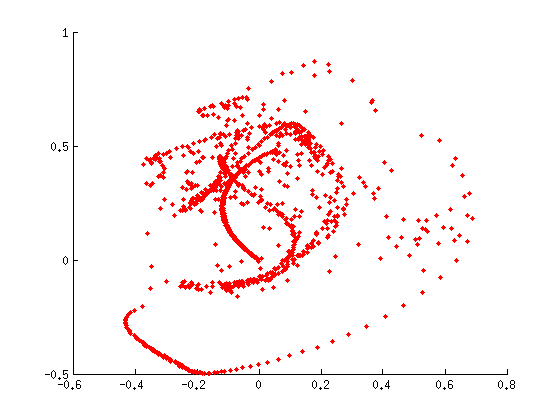
\includegraphics[width = 0.4\textwidth]{PeqDsect_refred3}
 (b) 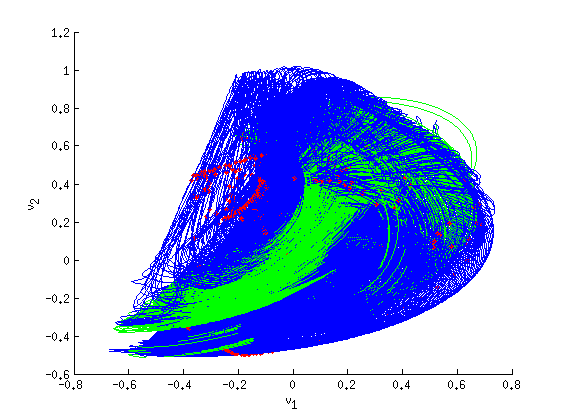
\includegraphics[width = 0.4\textwidth]{tw1manrefred3PeqDsect} \\
 (c) 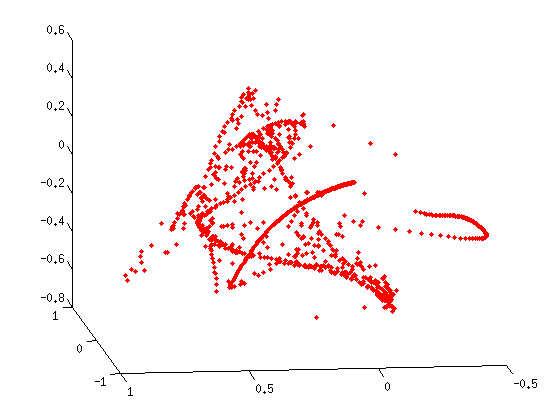
\includegraphics[width = 0.4\textwidth]{PeqDsect_refred3_angle2}
 (d) 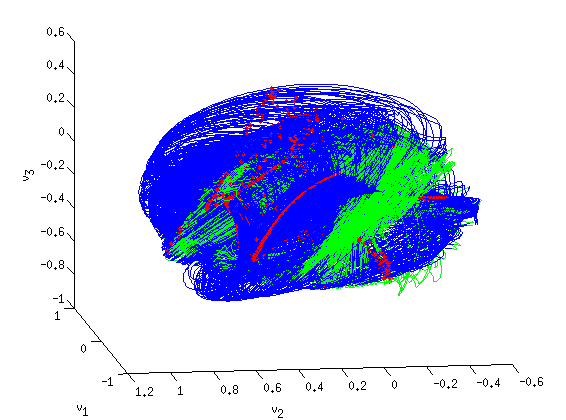
\includegraphics[width = 0.4\textwidth]{tw1manrefred3PeqDsect_angle2}
  \caption{Long \KS\ trajectories ($t_f = 200$) started on the unstable
  manifold of $\REQV{}{1}$ (c, d) where episodes with almost vanishing first
  mode are drawn green, captured from two different angles of 3D projections
  onto the unstable eigenvectors of $\REQV{}{1}$. Intersections of these trajectories
  with the \PoincSec\ defined by $P=D$ are marked with red on the
  figures themselves, and individually on (a) and (c) where (a) and (c) are
  snapshots from the same viewing angle with (b) and (d) respectively.
  }
  \label{f-tw1manrefred3}
\end{figure}

\begin{figure}[h]
  \centering
  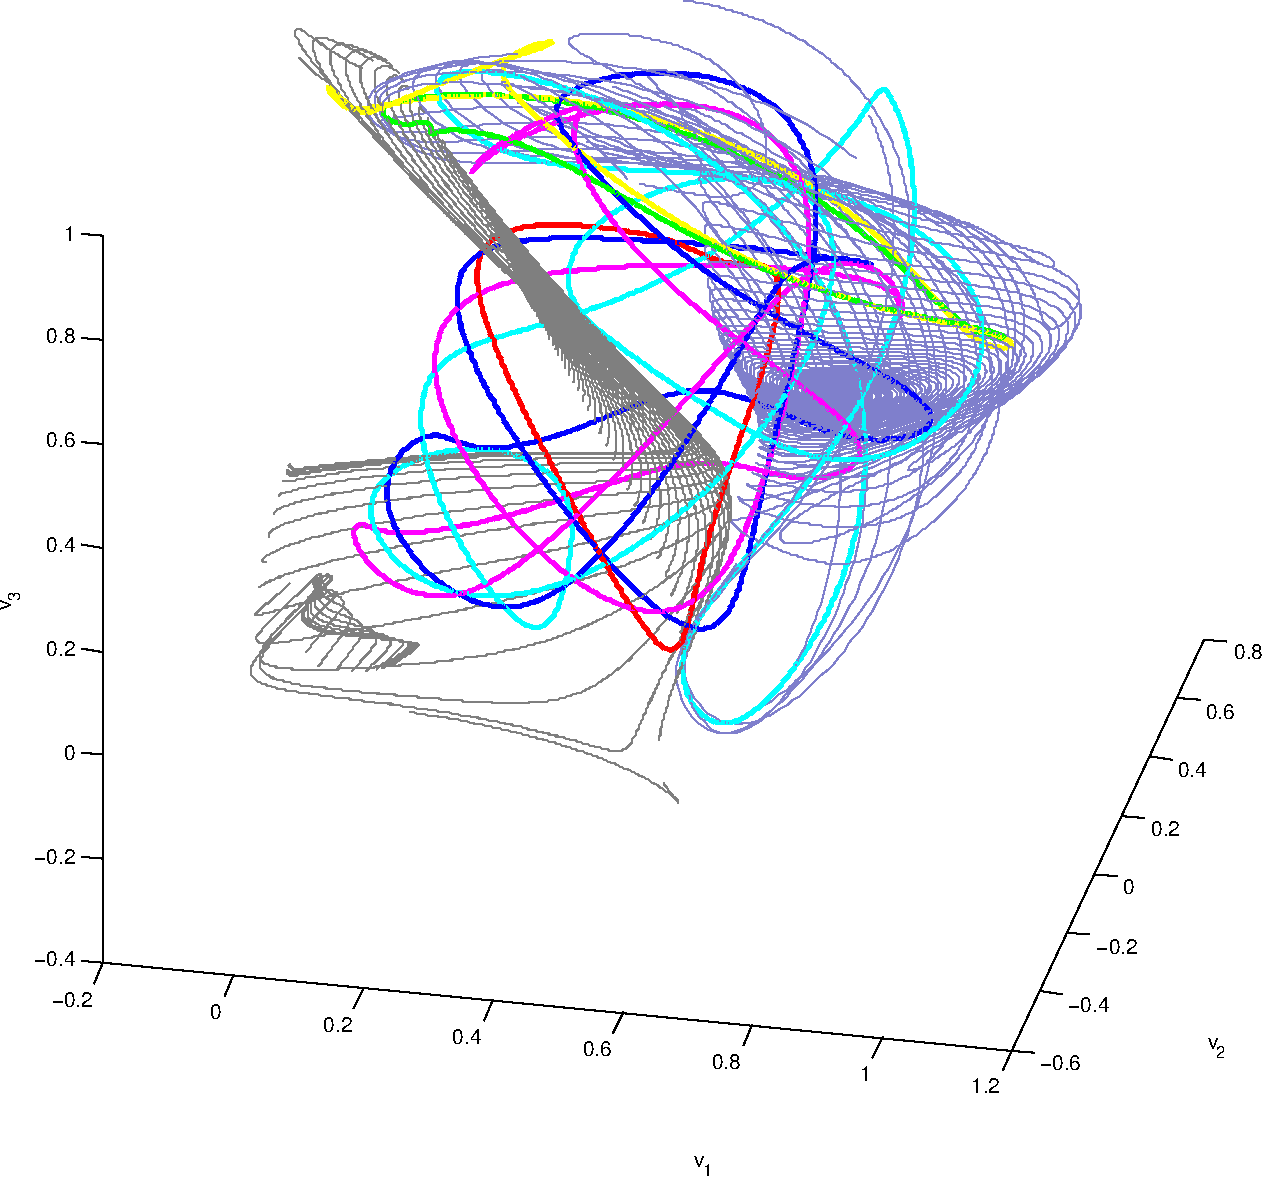
\includegraphics[width = 0.8\textwidth]{eq2tw1man3ppo3rpo}
  \caption{Unstable manifold of $\EQV{2}$ (gray) and $\REQV{}{1}$ (blue) located
  relative to $\EQV{2}$   (origin), and projected onto the basis constructed from
  the linear combinations of unstable eigenvectors of $\EQV{2}$ and $\REQV{}{1}$ and
  the vector which connects $\EQV{2}$ to $\EQV{3}$. Three relative and three pre
  periodic orbits are drawn on top of these manifold.}
  \label{f-eq2tw1man3ppo3rpo}
\end{figure}

Next thing I spent sometime looking at is the projection where I visualized
the unstable manifold of $\REQV{}{1}$ and $\EQV{2}$ together
\reffig{f-eq2tw1man3ppo3rpo}. Advantage of this projection is that we can see
which unstable manifold organizes which rpo/ppo. I looked at a plane
\PoincSec\ on this projection where I tried to capture both the region
of the unstable manifold of $\REQV{}{1}$ (close to the border), which seems to be
followed by some \po s and the connection between $\EQV{2}$ and $\EQV{3}$. With this
motivation, I picked a \PoincSec\ which involves the origin ($\EQV{2}$),
and makes $3 \pi / 8$ angle with the $v_1$ axis in \reffig{f-eq2tw1man3ppo3rpo}.
I then found the \PoincSec\ points of the 200 \rpo s and 200 \ppo s with this section
\reffig{f-psect_eq2tw1_400rpoppo}. All \rpo s and \ppo s intersect with this section
except the first \ppo\ \PPO{} (drawn red in \reffig{f-eq2tw1man3ppo3rpo}) which lies
outside the attractor, according to Xiong. First 200 \rpo s and \ppo s of the
\KS\ intersected this \PoincSec\ at maximum 9 times and parts of the
section in \reffig{f-psect_eq2tw1_400rpoppo} seems relatively thin.

While the projection \reffig{f-eq2tw1man3ppo3rpo} has been helpful in
visualizing manifolds together, I think I should look at two manifolds and
\PoincSec s on them individually. I'm thinking that it will only be
possible to reduce things to almost one dimension around the unstable
manifolds where the flow is almost two dimensional. Ultimately, I'm thinking
that one can categorize the periodic orbits in families, just as the pipe
team does, and then write the spectral determinant as a product over the
families, and thus expand `family by family' ensuring (at least, expecting)
shadowing.

\begin{figure}[h]
  \centering
  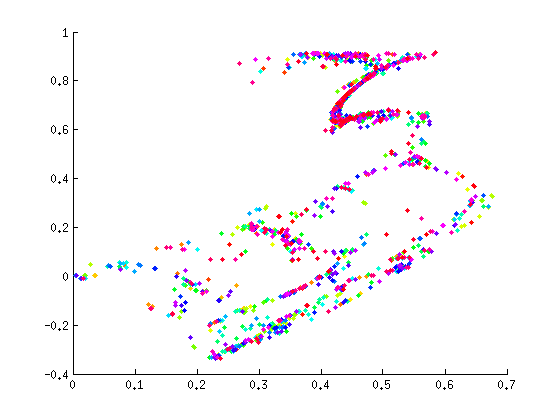
\includegraphics[width = 0.8\textwidth]{psect_eq2tw1_400rpoppo}
  \caption{Intersections of 200 \rpo s and 200 pre-periodic orbit with a plane
  \PoincSec\ within the projection visualized in
  \reffig{f-eq2tw1man3ppo3rpo}.}
  \label{f-psect_eq2tw1_400rpoppo}
\end{figure}

\item[2014-10-22 Predrag]
Now it is official:
\HREF{http://www.theonion.com/articles/historians-admit-to-inventing-ancient-greeks,18209/}
{Evangelos} does not exist. ``The Iliad was a bitch to write, by the way,''
Professor Gene Haddlebury continued, referring to the epic poem believed
to have laid the foundation for the Western literary tradition. ``But it
seemed to catch on.''

``We picked Greece because we figured nobody would ever go there to check
it out,'' Emily Nguyen-Whiteman said. ``Have you ever seen the place?
It's a dump. It's like an abandoned gravel pit infested with cats''

\item[2014-12-18 Burak]
Observing the developments in pipe group, I decided to project
symmetry-reduced (both translations and reflections) \KS\ dynamics onto
principal components. There are 9 figures in \reffig{f-ksPCAnpo}, all
showing a long ergodic trajectory, and the equilibria of the flow.
\refFig{f-ksPCAnpo} (b) shows two pre-periodic (green and cyan) and one
relative periodic orbits. From (c) to (i) I added 1 \ppo\ and 1 \rpo\ to the
next figure. My initial hope was to find a way to categorize periodic
orbits into families as done in the pipe. Looking at \reffig{f-ksPCAnpo},
I'm neither optimistic nor pessimistic about this. It starts promising when
there are three periodic orbits (\reffig{f-ksPCAnpo} (b)), two on the left
and one on the right; but starting with the fourth one, periodic orbits
visit both sides. I have already tried to look at the \PoincSec\ on
the two dimensional unstable manifold of the shortest \ppo\ (green orbit on
\reffig{f-ksPCAnpo} (b)), but I couldn't find anything like a set of points
organized on an almost one dimensional curve. So I don't know.

One interesting feature on \reffig{f-ksPCAnpo} is that the ergodic
trajectory visits the neighborhood of $\EQV{2}$ quite often. This is not the
case with other equilibria/traveling waves. I'm blogging
\reffig{f-ksPCAnpo} (a) from a different angle on \reffig{f-ksPCA} where
this is more obvious. I have also previously seen that the `almost
non-hyperbolic' periodic orbits of the \KS\ system were the ones which
visited the close neighborhood of $\EQV{2}$. So I'm thinking more and more
that may be we should include $\EQV{2}$'s contribution to the trace formulas.

\begin{figure}% [h]
\begin{center}
   (a) 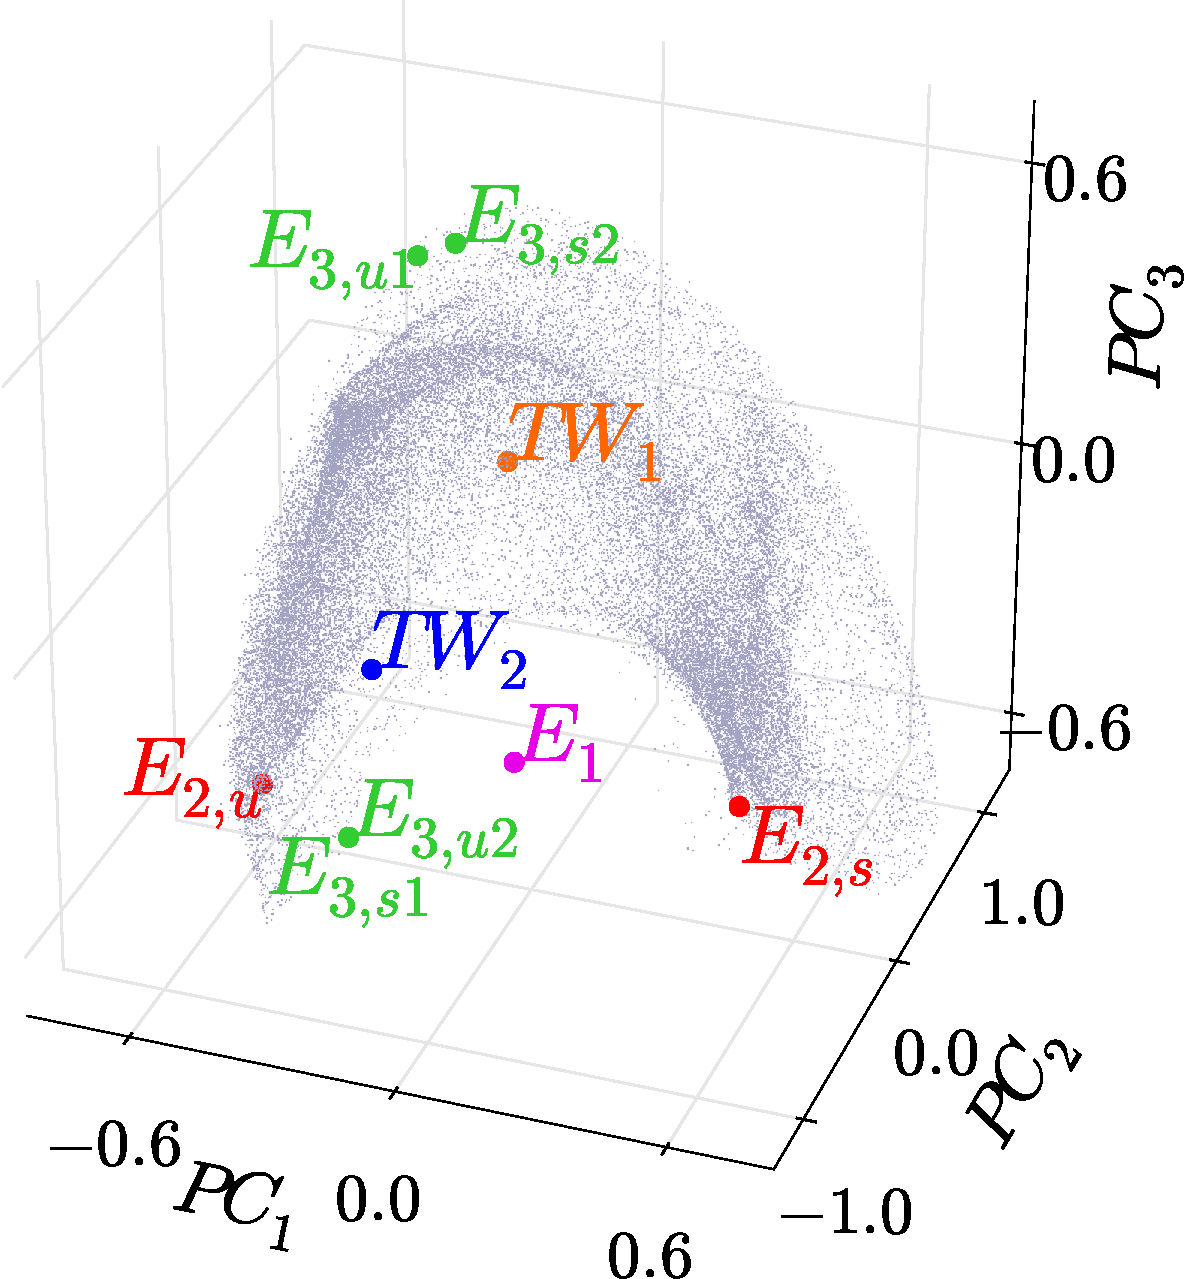
\includegraphics[width = 0.26\textwidth]{ksPCA0po}
   (b) 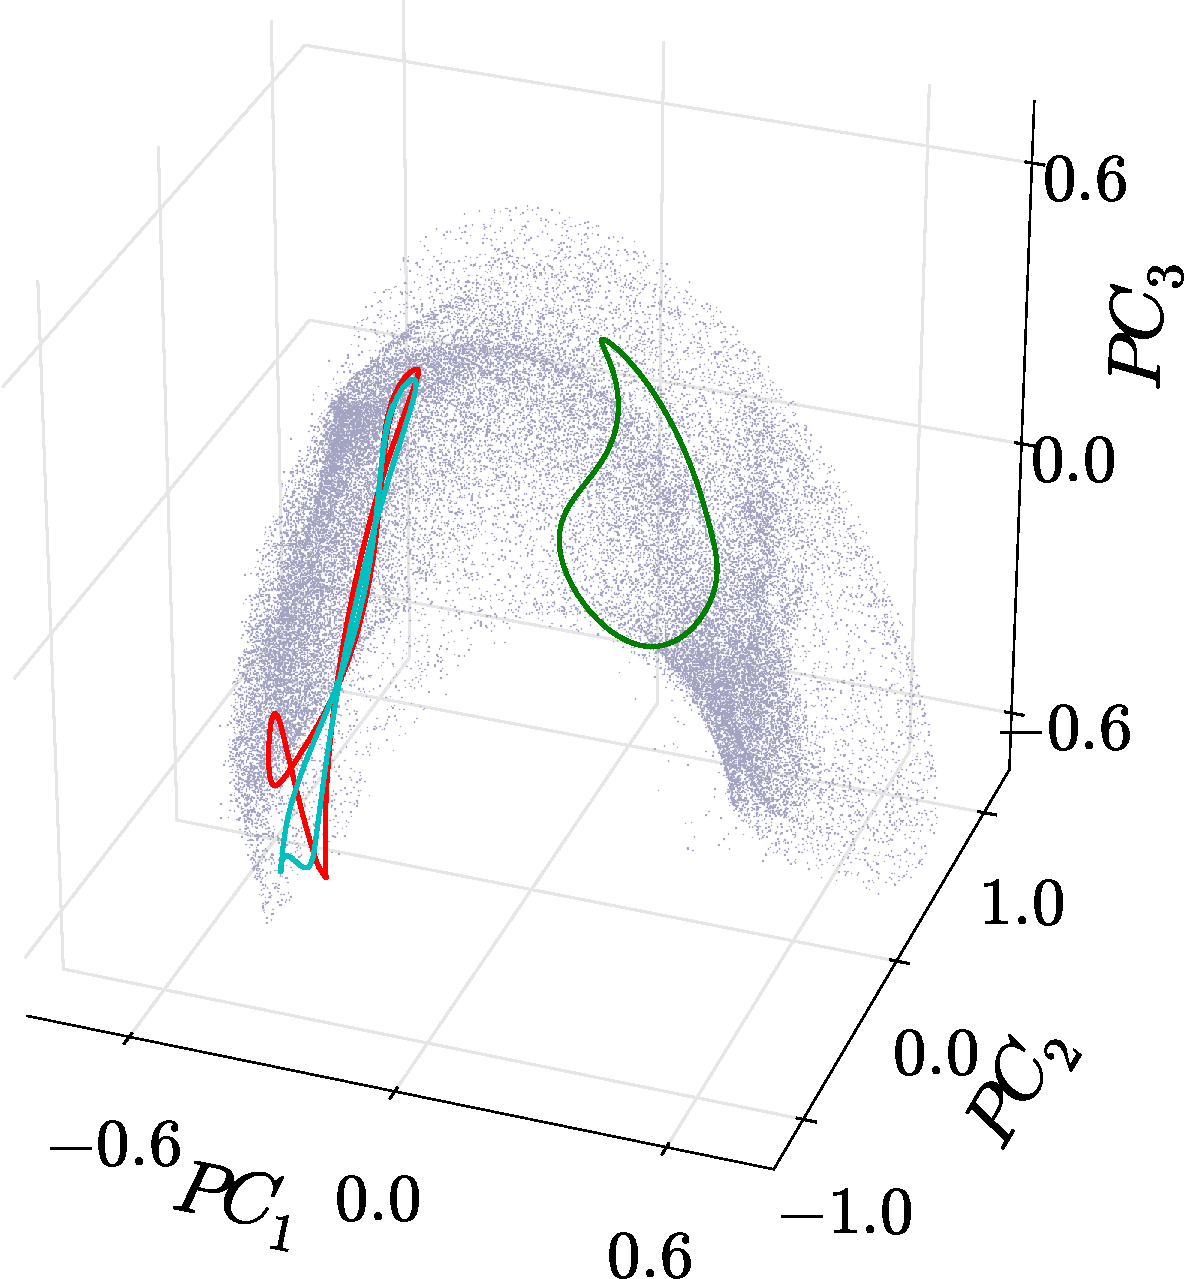
\includegraphics[width = 0.26\textwidth]{ksPCA3po}
   (c) 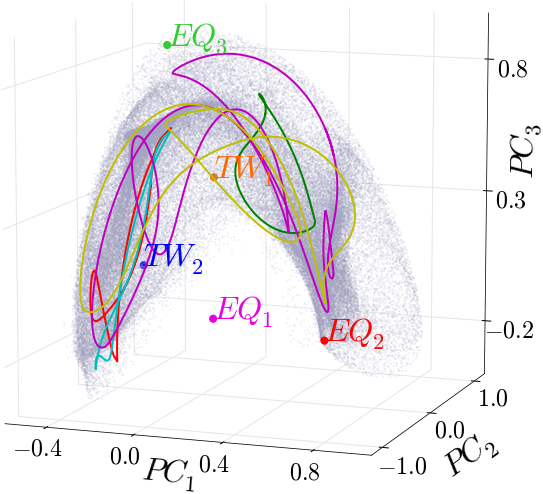
\includegraphics[width = 0.26\textwidth]{ksPCA5po} \\
   (d) 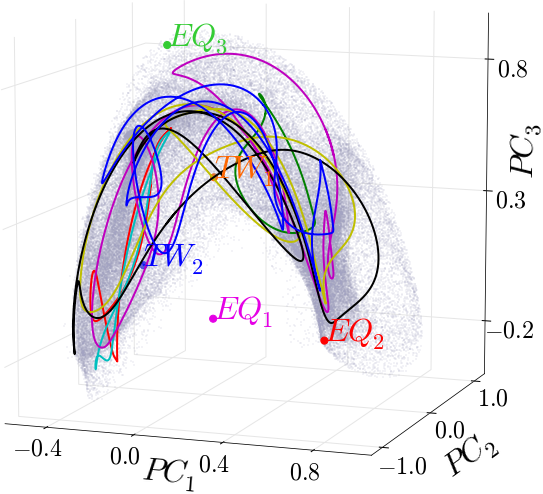
\includegraphics[width = 0.26\textwidth]{ksPCA7po}
   (e) 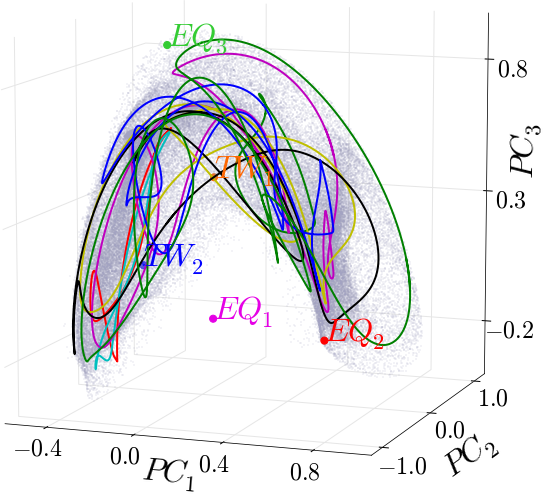
\includegraphics[width = 0.26\textwidth]{ksPCA9po}
   (f) 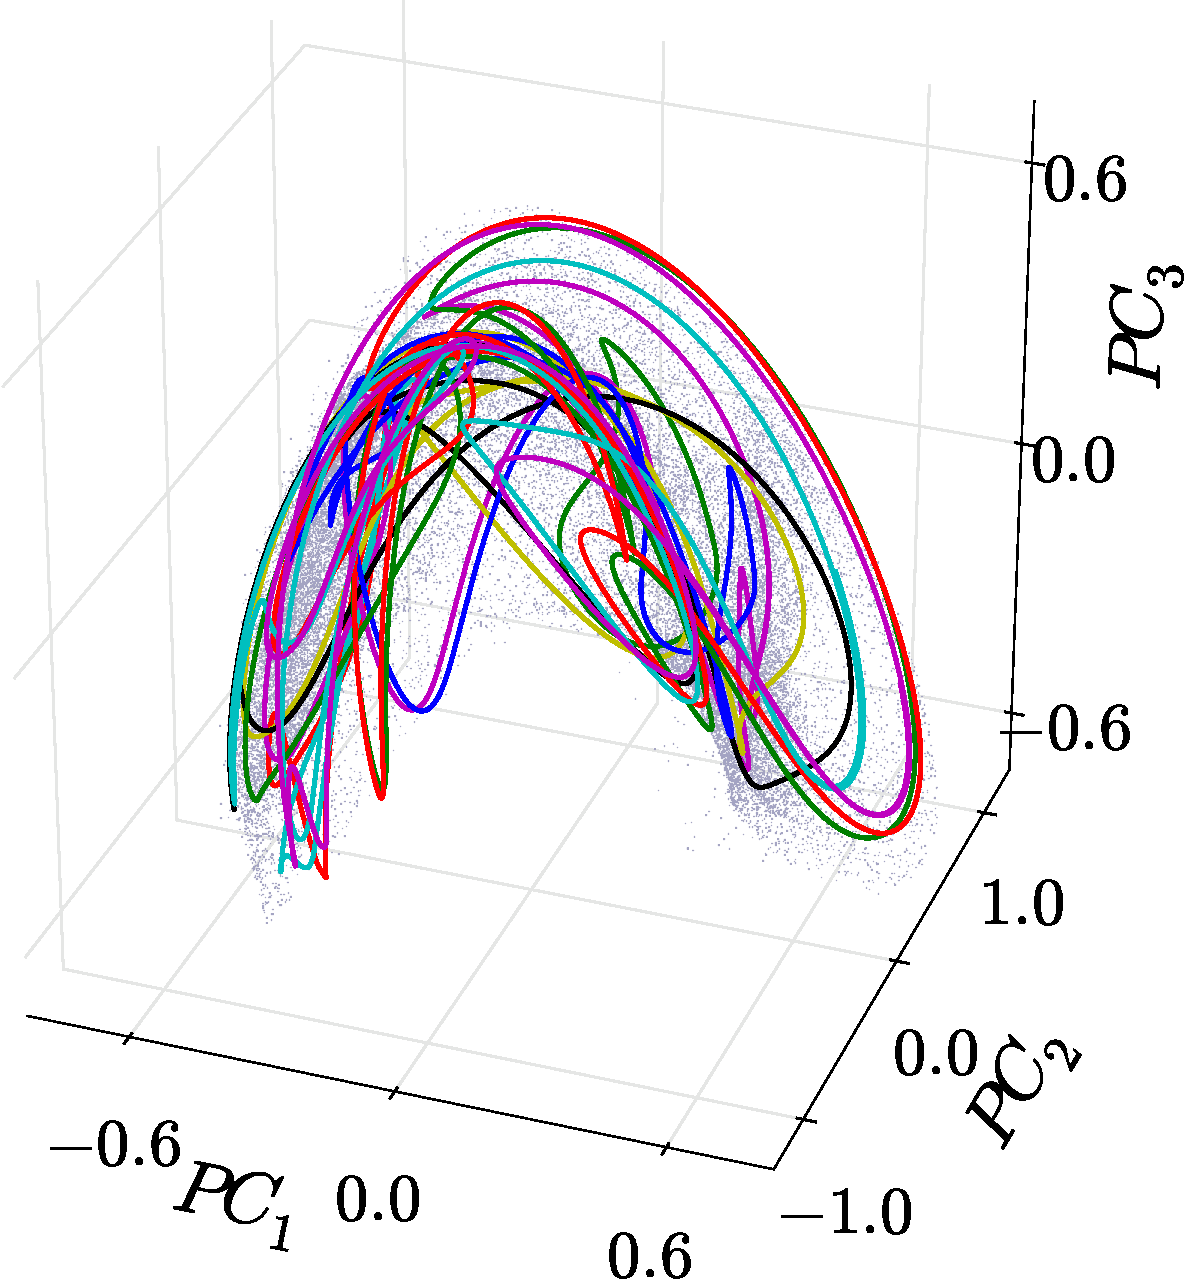
\includegraphics[width = 0.26\textwidth]{ksPCA11po} \\
   (g) 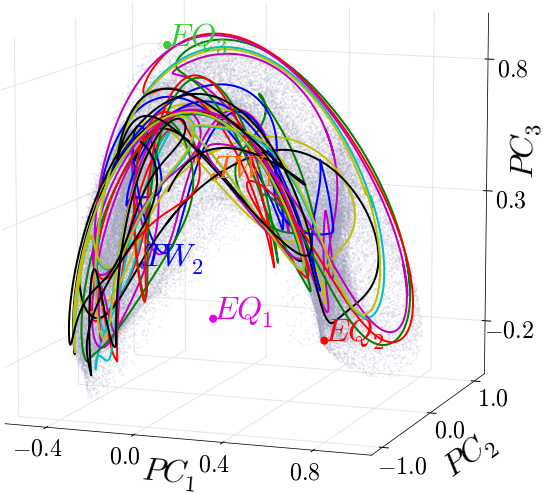
\includegraphics[width = 0.26\textwidth]{ksPCA13po}
   (h) 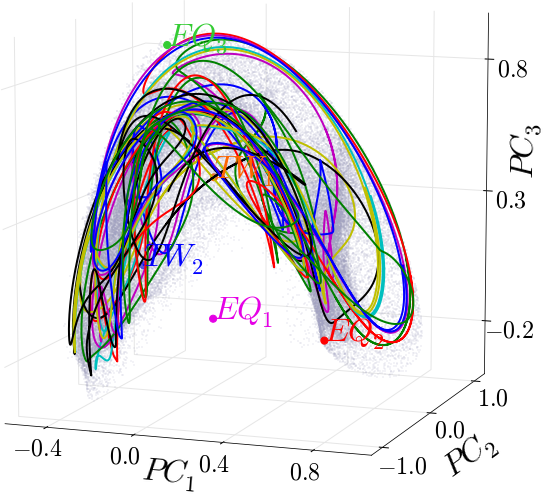
\includegraphics[width = 0.26\textwidth]{ksPCA15po}
   (i) 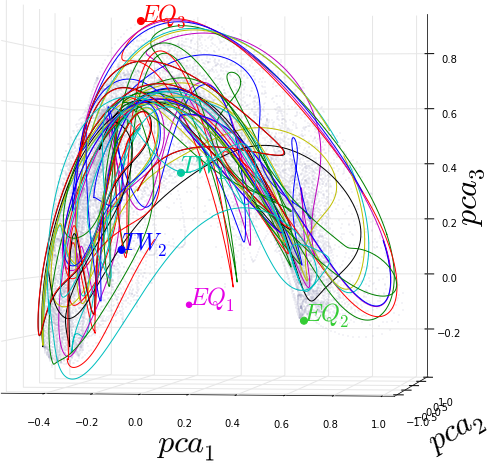
\includegraphics[width = 0.26\textwidth]{ksPCA17po}
\end{center}
   \caption{(a) Equilibria, traveling waves and a long ergodic
         trajectory (gray dots) of the \KS\ system projected
         onto leading three principal components obtained
         from PCA of the ergodic trajectory.
         (b) Same as (a), with addition of 2 PPO, 1 RPO,
         (c) Same as (a), with addition of 3 PPO, 2 RPO,
         (d) Same as (a), with addition of 4 PPO, 3 RPO,
         (e) Same as (a), with addition of 5 PPO, 4 RPO,
         (f) Same as (a), with addition of 6 PPO, 5 RPO,
         (g) Same as (a), with addition of 7 PPO, 6 RPO,
         (h) Same as (a), with addition of 8 PPO, 7 RPO,
         (i) Same as (a), with addition of 9 PPO, 8 RPO.
         }
  \label{f-ksPCAnpo}
\end{figure}


\begin{figure}[h]
  \centering
  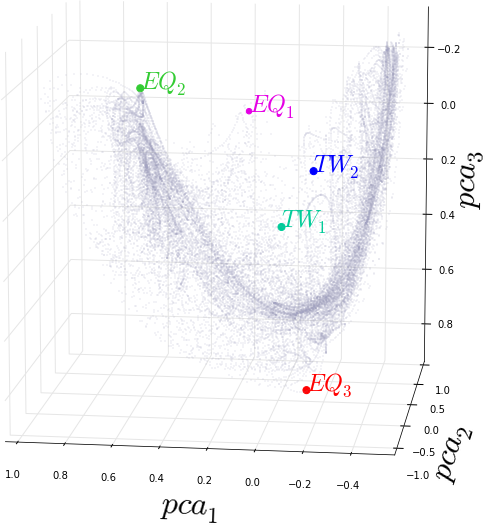
\includegraphics[width = 0.8\textwidth]{ksPCA}
  \caption{Ergodic trajectory and the equilibria of the \KS\ system on
         the PCA coordiates.}
  \label{f-ksPCA}
\end{figure}

\item[2014-12-19 Burak] I thought a little bit about these and I started to
believe that doing PCA to turbulent data in whatever coordinates one has
doesn't really mean much. Especially in the case of \KS , I'm first
transforming to the first Fourier mode slice, and then applying
\refeq{e-xRefs3}; so god knows what's the proper final metric. In the
language of PCA, it's said that "PCA is sensitive to the scaling of the
data", which I think corresponds to the choice of the metric for our case.
So I decided to learn `Sobolev norms' and I'll try to figure out how does
the corresponding metric transform during the coordinate transformations.

\item[2016-03-23 Xiong] :

{\bf \FFslice} reduction of \On{2}
is defined by rotation into
\beq
\Re(\hat{a}_1) = 0 \,\quad \Im(\hat{a}_1) > 0
\ee{XDfFslice}
and, if needed, the reflection to bring the \statesp\ point into the
fundamental domain $\Re(\hat{a_2}) > 0$.

The physical problem with the  \fFslice\ that \KS\ for $L=22$ has a weak
first Fourier mode: the dynamics on the attractor is a competition between
the second and third modes. So my intuition is that the \sFslice\ would be
better, with fewer excursion close to the {slice border}, as the \EQV{2}
unstable manifold dominates the dynamics.

 {\bf \SFslice} reduction of \On{2} is defined by rotation into
\beq
b_2 = 0 \,\quad c_2 > 0,
\,,
\ee{XDsFslice}
where $\hat{a}_k = b_k+ic_k$. With this choice the reflection
\refeq{XDsFsliceRefl} does not change its rule  after reducing $\SOn{2}$.

Due to the phase wrapping of the second Fourier mode,  after the
\refeq{XDsFslice} reduction of \SOn{2}, in the {\reducedsp} the system
has an additional discrete symmetry,
$C_{2v} = C_{2v}\times C_{2v}$:
\bea
  a_k  &\to& -a^*_k     \label{XDsFsliceRefl}\\
  a_k  &\to& e^{ik\pi} a_k  \label{XDsFsliceShift2}
\,.
\eea
Here I construct a fourth order invariant polynomial to reduce $C_{2v}$
(for a reduction without polynomials, see \refeq{XDsFslice}).
The first step is
\[
  [a_1, a_2, a_3, a_4, a_5, \cdots] \to
  [a^2_1, a_2, a_3a_1, a_4, a_5a_1, \cdots]
\,.
\]
The odd terms are multiplied by $a_1$, thus the \sFslice\ induced $C_2$
symmetry \refeq{XDsFsliceShift2} is reduced.
Denote the state now to be $[\bar{a}_1, \bar{a}_2, \cdots]$.
From $\bar{a}_1$ we can recover 2 distinct $a_1$, and from each $a_1$, the
remaining $a_{2k+1}$ follow.  Now reflection \refeq{XDsFsliceRefl} takes form
\beq
  [\bar{a}_1, \bar{a}_2, \bar{a}_3, \bar{a}_4, \bar{a}_5, \bar{a}_6,\cdots]
  \to
  [\bar{a}^*_1, -\bar{a}^*_2, \bar{a}^*_3, -\bar{a}_4, \bar{a}^*_5, -\bar{a}^*_6,\cdots]
\ee{BB1stSlRefl}
So odd terms flip the sign of imaginary part, and even terms flip the sign
of real part. Gather the part which change sign :
$[\bar{c}_1, \bar{b}_2, \bar{c}_3, \bar{b}_4, \cdots]$. Then following transformation
reduces reflection:
\beq
  [\bar{c}_1, \bar{b}_2, \bar{c}_3, \bar{b}_4, \cdots] \to
  [\bar{c}_1^2, \bar{b}_2\bar{c}_1, \bar{c}_3\bar{c}_1, \bar{b}_4\bar{c}_1, \cdots]
\ee{XDD4reduc}
These polynomials are 4th order.

\refFig{fig:ksE2Wu} shows the
unstable manifold of \EQV{2} and the first 100 \ppo s and \rpo s.

What I found interesting is that after reducing \On{2}, the first 6
eigenvectors of \EQV{2} all vanish. It seems that a large part of the
tangent space of \EQV{2} collapses to point \EQV{2}. The discontinuity in
\reffig{fig:ksE2Wu}\,(a) is the part closed to ``slice'' boarder.
$\RPO{1}=\RPO{16.32}$ is picked out because it is frequently shadowed by other
orbits.
Comparing (a) with (b), it seems that the set of \po s is shadowing the
unstable manifold of \EQV{2} and $\RPO{1}=\RPO{16.32}$.

\begin{figure}[h]
  \centering
  (a)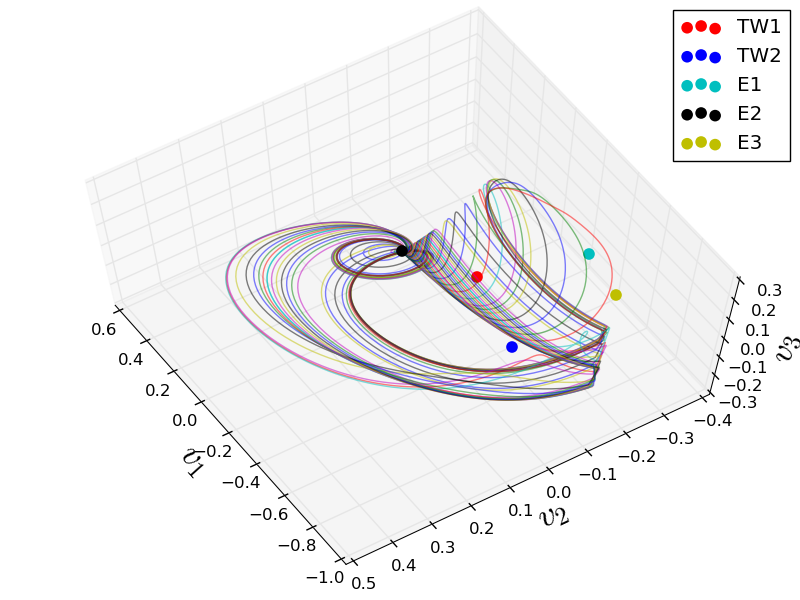
\includegraphics[width=0.46\textwidth]{ksE2Wu}
  (b)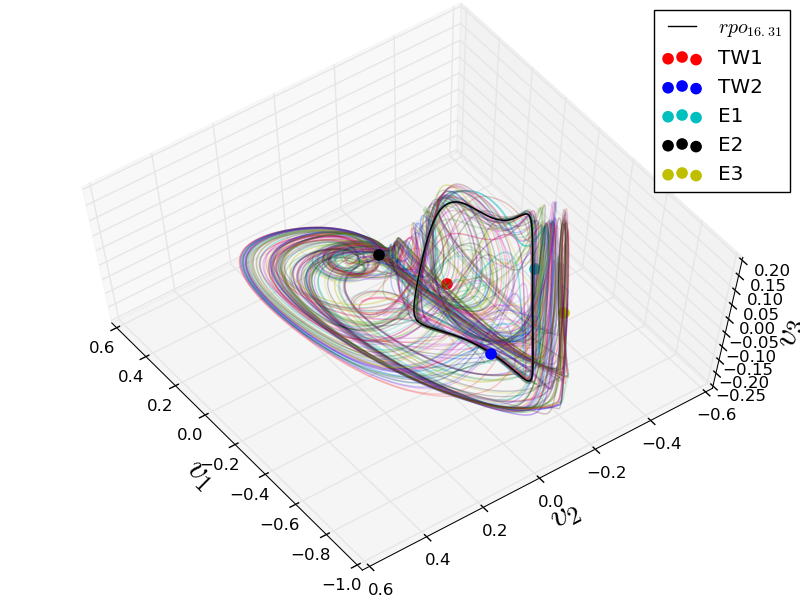
\includegraphics[width=0.46\textwidth]{ksPO50}
  \caption{
    \SFslice\ + invariant polynomial \refeq{XDD4reduc} reduction of \On{2}.
    (a) Unstable manifold of \EQV{2}. (b) first 50 \rpo s and first 50 \ppo s.
    Orthogonal bases
    $v_1$ and $v_2$ and $v_3$ are constructed from eigenvectors of \EQV{2}
    $e_{7,R}$, $e_{7, I}$ and
    $e_{11, R}$ in the symmetry reduced space.
  }
  \label{fig:ksE2Wu}
\end{figure}

\item[2016-03-24 Xiong] Based on the profile in \reffig{fig:ksE2Wu}, I
tried to construct a \PoincSec\ which can capture the essential
dynamics. The \PoincSec\ is perpendicular to the x-y plane, and
has two sectors which join at \EQV{2}. The reason that I use two
half planes joined not with angle $\pi$ is that I think this system
is different from 2modes or Rossler system we have encountered before.
Here \EQV{2} is an equilibrium, but it is actually a point on an infinite
many \po s since its unstable manifold form homoclinic orbits.
So different sectors are used to capture trajectories going in to
and going out from \EQV{2}.

\refFig{fig:ksPoinc} shows the \PoincSec\ points for
ergodic trajectory and ppo/rpos. The \PoincSec\ points form
thin curves. We may produce a good return map. Note, the upper
left part of panel (d) is different from that of (c) because
ppo/rpos frequently shadow $\RPO{1}=\RPO{16.32}$, but the ergodic trajectory
seems not interested in $\RPO{1}=\RPO{16.32}$. This confuses me.

\item[2016-03-28 Predrag]
What is the precision of the \cLvs\ algorithm?
Are there more digits in $\lambda_4= -0.003xxx$ for which you trust numerics?
It is hard to tell from \reftab{DingCvit14:floquet_ppo1}.
In \texttt{lyapunov/KS.tex}, {\bf [2009-09-13 Ruslan]} also gives
$\lambda_4= -0.003$.
(To see the above references, compile \texttt{lyapunov/blog.tex}
without \texttt{inclOnly.tex} lines commented out.)
Exponent $\lambda_4= -0.003$ is way too close to zero to be accidentally
so small, other \entangled\ modes have $\lambda_j \approx \pm 0.1$, see
\reftab{DingCvit14:floquet_ppo1}. Does it have something to do with
`misaligned' marginal modes:
\(
\eigRe[3]_{10.25}= \eigRe[4]_{10.25} = 0
\,,
\)
but
\(
\eigRe[2]_{16.31}= \eigRe[3]_{16.31} = 0
\,?
\)
Is there a close-by bifurcation in $L=22$ ($L=22$  is merely a random system
size empirically chosen by Evangelos, Ruslan, and me)?

The problem is that we should not only be pairing modes by their
approximate \On{2} degeneracy, but also not label \entangled\ modes by
the order of magnitude of their $\eigRe[j]_{p}$, but by the properties of
their eigenvectors. That will become a necessity when we look at large
$L$ \KS\ systems. I suspect the correct pairing is
\beq
\eigRe[1]_{16.31}= 0.32791
\,,\quad
\eigRe[2]_{16.31} = -0.13214
\,,\quad
\eigRe[3]_{16.31}= \eigRe[4]_{16.31} = 0
\,.
\ee{16.31leadFloq}
Note also that in the above {\bf [2016-03-24 Xiong]} observes that
$\RPO{1}=\RPO{16.32}$ is NOT embedded into the long-time ergodic
attractor, instead it seems to be the backbone of a transient repeller
Smale horseshoe. Indeed, this might explain why its exponents are so
different from the Lyapunov exponents. However, I'm for keeping it in the
paper, as it is still embedded in the inertial manifold. The
fractional-dimension strange attractor is a very structurally unstable
set, but the smooth, integer dimension inertial manifold enveloping it
should be robust.


%%%%%%%%%%%%%%%%%%%%%%%%%%%%%%%%%%%%%%%%%%%%%%%%%%%%%%%%%%%%%%%%%%%%%%%
\begin{table}[h]
  \footnotesize
  \begin{center}
  \caption{
    The first 10 Floquet multipliers
    $ \ExpaEig_i= \exp(\period{}\,\eigRe[i] \pm i\theta_{i})$ for
    orbits $\PPO{10.2}$ and $\RPO{1}=\RPO{16.32}$, respectively.
    $\theta_{i}$ column lists either the phase,
    if the Floquet multiplier is complex, or `-1' if the
    multiplier is real, but inverse hyperbolic. Truncation number
    $N=64$. Extracted from \refref{DingCvit14}.
  }
  \label{DingCvit14:floquet_ppo1}
  \begin{tabular}{l l c | l l c}
    \multicolumn{3}{c |}{$\PPO{10.2}$} & \multicolumn{3}{c}{$\RPO{1}=\RPO{16.32}$}\\
    $i$ & ~~~~~$\eigRe[i]$  & $\theta_{i}$  & $i$ & ~~~~~$\eigRe[i]$ & $\theta_{i}$  \\
    \hline
    1,2 & ~0.033209  &    $\pm$2.0079  &  1 &     ~0.32791  &              \\
    3 & -4.1096e-13  &                 &  2 &   ~2.8679e-12  &              \\
    4 & -3.3524e-14  &    -1           &  3 &   ~2.3559e-13  &              \\
    5 &  -0.21637    &                 &  4 &     -0.13214  &        -1    \\
    6,7 &  -0.26524  &   $\pm$2.6205   &  5,6 &   -0.28597  & $\pm$2.7724  \\
    8 &  -0.33073    &    -1           &  7 &     -0.32821  &       -1     \\
      &              &                 &  8 &      -0.36241  &             \\
    9 &  -1.9605    &                  &  9 &    -1.9617   &  +2.2411   \\
    10 & -1.9676    &    -1            &  10 &   -1.9617  &  -2.2411 \\
    $\cdots$ &  $\cdots$    & $\cdots$ & $\cdots$ & $\cdots$ & $\cdots$   \\
%    \hline
\end{tabular}
\end{center}
\end{table}
%%%%%%%%%%%%%%%%%%%%%%%%%%%%%%%%%%%%%%%%%%%%%%%%%%%%%%%%%%%%%%%%%%%%%%%

%%%%%%%%%%%%%%%%%%%%%%%%%%%%%%%%%%%%%%%%%%%%%%%%%%%%%%%%%%%%%%%%%%%%%%%
\begin{figure}
\begin{center}
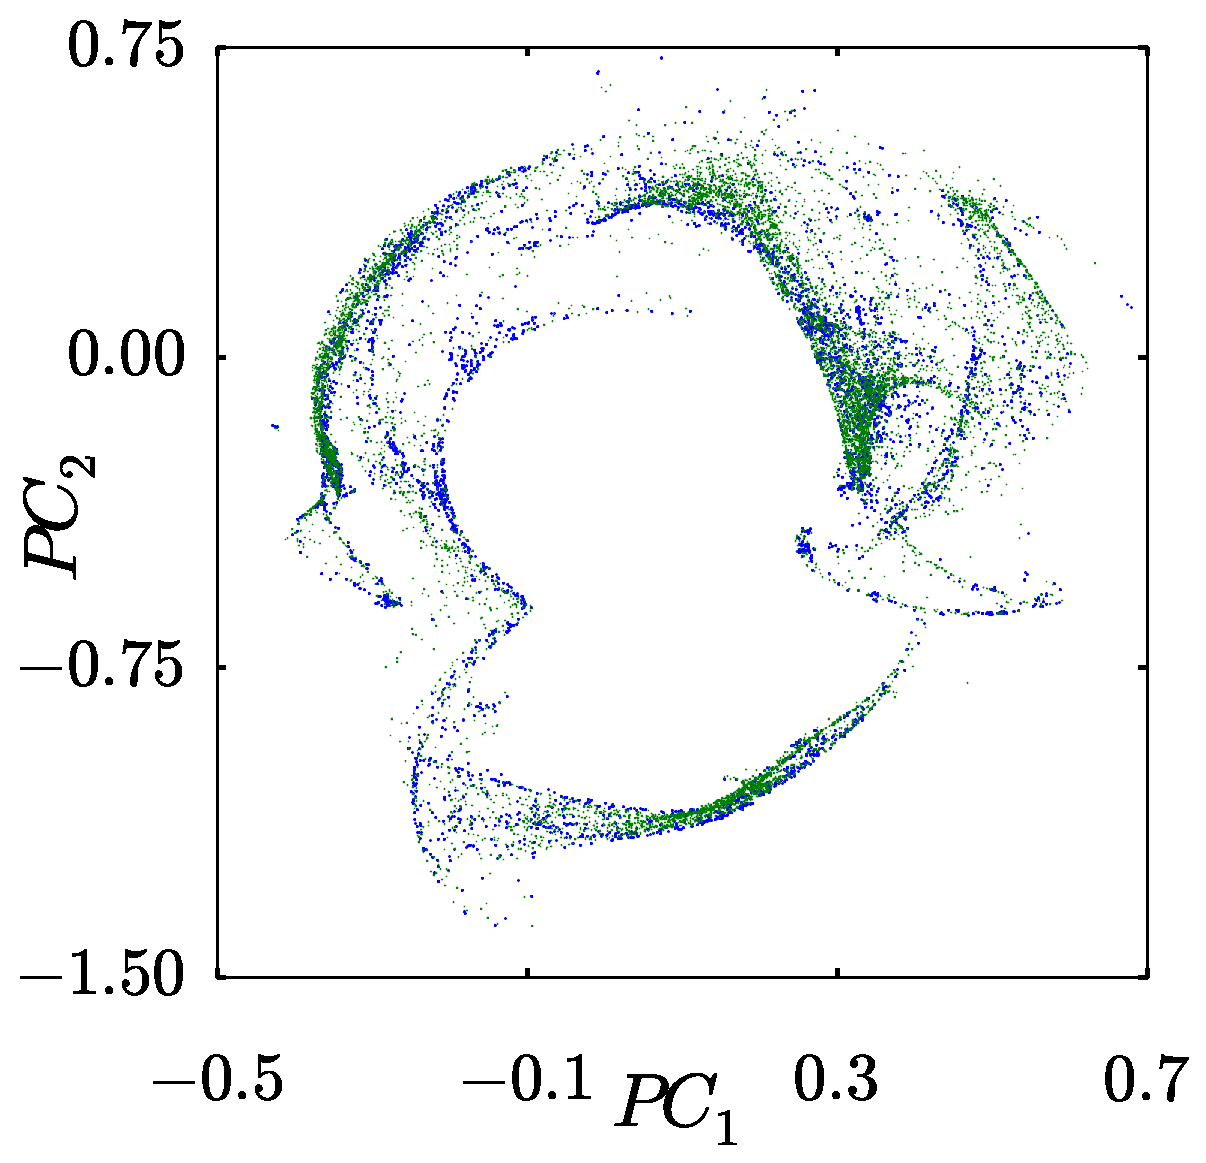
\includegraphics[width=0.95\textwidth]{ksPsectonPCA_POandErgodic}
\end{center}
\caption[]{
(Color online)
Intersections of the long ergodic trajectory (green) and $479$ \po s
(blue) with the \PoincSec\ which includes $\REQV{}{1}$ and is parallel to
$(PC_1, PC_2)$ plane. (From \refref{BuDiCv15})
}
\label{f-Poincare}
\end{figure}
%%%%%%%%%%%%%%%%%%%%%%%%%%%%%%%%%%%%%%%%%%%%%%%%%%%%%%%%%%%%%%%%%%%%%%%

%%%%%%%%%%%%%%%%%%%%%%%%%%%%%%%%%%%%%%%%%%%%%%%%%%%%%%%%%%%%%%%%%%
\begin{table}[t]
\caption{
Leading eigenvalues
$\eigExp[j]= \eigRe[j] \pm i\eigIm[j]$
and symmetries of the corresponding eigenvectors
of KS \EQV{2} for $L = 22$ system size.
We have used as our reference states the ones that lie within
the antisymmetric subspace  $\bbU^+$,
and also listed the symmetries of
the $L/4$ translated ones. See \reftab{tab:Eksym}.
        }\label{tab:EksymE2}
\begin{center} \footnotesize
\begin{tabular}{ccccc}
\EQV{2}&  &  & \\\hline
  $\eigExp[1,2]$ & $\ \ 0.1390$& $0.2384$ & $\bbU^+$         & $\bbU^{(1)}$\\
  $\eigExp[3]$   & $0$      &          & $\Shift_{1/2}$        & $\Shift_{1/2}$\\
  $\eigExp[4,5]$ &$-0.0840$ & $0.1602$ & $\bbU^{(1)}$           & $\bbU^+$\\
  $\eigExp[6]$   &$-0.1194$ &          & $\Shift_{1/2}$        & $\Shift_{1/2}$\\
  $\eigExp[7,8]$ &$-0.2711$ & $0.3563$ & $\bbU^+,\,\bbU^{(1)},\,\Shift_{1/2}$  & $\bbU^+,\,\bbU^{(1)},\,\Shift_{1/2}$\\
  $\eigExp[9]$   &$-2.0130$ &          & $\bbU^{(1)}$           & $\bbU^+$\\
  $\eigExp[10]$  &$-2.0378$ &          & $\bbU^+$         & $\bbU^{(1)}$\\[2ex]
\end{tabular}
\end{center}
\end{table}
%%%%%%%%%%%%%%%%%%%%%%%%%%%%%%%%%%%%%%%%%%%%%%%%%%%%%%%%%%%%%%%%%%

\item[2016-04-08 Predrag to Xiong] I do not like that we have gone to 4th
order polynomials \refeq{XDD4reduc} and $e_{7,R}$, $e_{7, I}$, and
$e_{11,R}$ (11!) stability vectors; would have preferred leading vectors from
\reftab{tab:EksymE2}.

Think of $x^4$: it makes anything $<1$ nearly
zero, and blows up anything $>1$. One would like to avoid such
deformations - one of the reasons why we slice rather than use invariant
polynomials.

That after Xiong's 2nd Fourier mode slice for \On{2}, the first 6
eigenvectors of \EQV{2} vanish might be ``interesting,'' but is sure ulcer
inducing. Hopefully 1 of them is the spatial translation marginal
eigenvector, so that leaves us with 5 leading (!) Floquet modes
``vanishing''.

According to the bifurcation diagram \reffig{fig:ksBifDiag}, %{fig:GreeneKim},
$\EQV{2}$ is a $2$-cell state.

%%%%%%%%%%%%%%%%%%%%%%%%%%%%%%%%%%%%%%%%%%%%%%%%%%%%%%%%%%%%%%%%
\begin{figure}[t]       \label{fig:ksBifDiag}
\begin{center}
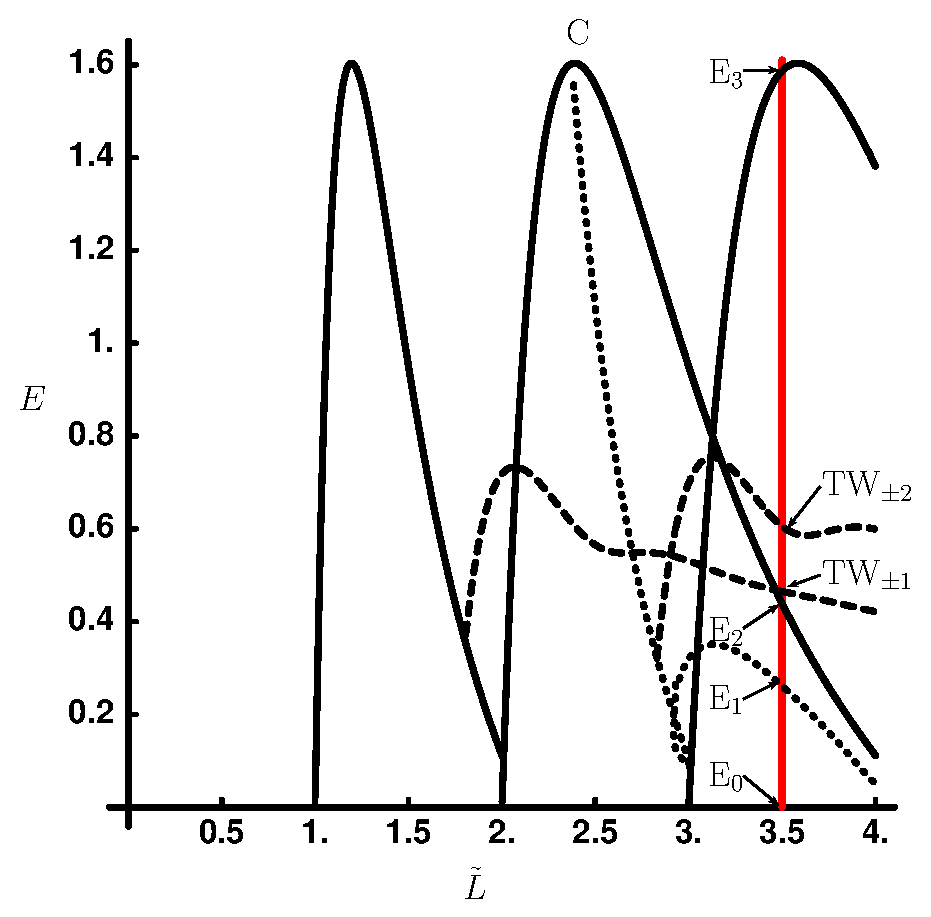
\includegraphics[width=0.5\textwidth]{ksBifDiag}
\end{center}
\caption{
The energy %\refeq{ksEnergy}
of the \eqva\ and \reqva\ that
exist up to $L=22$, $\tildeL = 3.5014\ldots$, plotted as a function
of the system size $\tildeL = L/2\pi$ (additional \eqva, not present
at $L = 22$ are given in \refref{ksgreene88}). Solid curves denote
$n$-cell solutions \EQV{2} and \EQV{3}, dotted curves the GLMRT
\eqv\ \EQV{1},
and dashed curves the \reqva\ \REQV{\pm}{1} and \REQV{\pm}{2}.
The parameter $\alpha$ of \refrefs{KNSks90,ksgreene88} is
related to the system size by $\tildeL=\sqrt{\alpha/4}$.
        }
\end{figure}
%%%%%%%%%%%%%%%%%%%%%%%%%%%%%%%%%%%%%%%%%%%%%%%%%%%%%%%%%%%%%%%%%%



The unstable manifold of the \EQV{2}
has a \hec\ to itself  shifted by
$L/2$, and \EQV{3} unstable manifold has a \hec\ to \EQV{2}.
Why does all of the unstable manifold of
\EQV{2}~\eqv\ go back
into
\EQV{2}~\eqv?
That makes for a rigid backbone and might provide a clue for how to
partition symbolic dynamics.
A correct symmetry reduction should identify
$\EQV{2}$ and its translated copy $\tau_{1/4}\EQV{2}$.
\EQV{2} and its unstable eigenvectors
happen to sit in the antisymmetric subspace
(recheck...), so \hec s should reflect these multiplicities.

Might want to have a look back at \reffig{f:KS22E2man1},
\reffig{f:ks22_E2_inv},
\reffig{f:ks22_E2_manif_rpo_homo},
\reffig{f:ks22_TW1_manifold},
\reffig{fig-2009-08-29TW1},
\reffig{f:KS22E2man1_copy},
and
\reffig{f:KS22E2man1_unwrapped}
.
And here are some earlier related discussions:

{\bf [2011-11-20 Ruslan]}:
\EQV{2} lives in $L/2$-periodic subspace, respectively.  To map it onto
$\pS/\On{2}$, we'll use the 2nd Fourier mode.
Once
$\EQV{2}$ is placed within $\pS/$\On{2} using the 2-nd Fourier
mode, its unstable manifold completely lives in the
anti-symmetric subspace (i.e. $Re\,a_k = 0$).
The manifold we show in our SIADS Fig.~5.6 is already in
$\pS/$\On{2}.  What worries me is that $\EQV{2}$ is represented
here by two different points ($\EQV{2}$ and
$\tau_{1/4}\EQV{2}$).  This is the result of the additional
symmetry of $\EQV{2}$.  Whether or not these two points can
be merged into one $\EQV{2}$ without loss of dynamical
information about the KS flow, remains to be investigated.
If we only look at KS solutions within the antisymmetric subspace, then
$\EQV{2}$ and $\tau_{1/4}\EQV{2}$ are two \underline{distinct}
equilibria, since the first one is unstable, while the second one is
stable.  So, there is no way to map these two equilibria into the same
point while staying within the antisymmetric subspace.
The \EQV{2} unstable manifold in the slice indeed looks like reduced
by $\Dn{1}$, but this is because the manifold is antisymmetric (i.e., lives
in $\mathbb{U}^+$, i.e. $b_k = 0$), so points on the manifold have either
$\theta_1 = \pi/2$, i.e. $c_1 > 0$, so do not need translation (i.e.
$\theta(a) = 0$), or $\theta_1 = -\pi/2$, i.e. $c_1 < 0$, for which
$\theta(a) = \pi$.

{\bf [2011-11-21 Ruslan]}:
in my original proposal for \On{2}
    symmetry reduction we never need anything more than the 1-st Fourier
    mode.  This is because points cannot be mapped into the $\theta =
    \pi/2$ slice only when both $r_1 = 0$ and $\dot{r}_1 = 0$.  But these
    conditions define the $L/2$ periodic solutions, which are invariant
    under \KS dynamics and thus appear only as limiting states.

{\bf [2011-11-21 Evangelos]} In \reffig{f:ks22_E2_inv}
$\EQV{2}$ and $\tau_{1/4} \EQV{2}$ are identified
and their connections become homoclinic. The unstable manifold of
$\EQV{2}$ has indeed been distorted nonlinearly and spiraling is not as
clear in \reffig{f:ks22_E2_inv} as in \reffig{f:ks22_E2_MSO2}. Moreover,
identification of $\EQV{2}$ and $\tau_{1/4} \EQV{2}$ makes the figure
more busy (unstable and stable manifolds lead to the same point).

{\bf [2011-11-24 Ruslan 2 Predrag]}
It is clear that dynamics on the chaotic attractor is dominated by the
unstable manifold of \EQV{2}, which is antisymmetric.

{\bf [Ruslan: 2009-10-17]}
... my hope was that the antisymmetric subspace would belong
to $\pS/\SOn{2}$.
The phase of the 1st Fourier mode is doing the job quite
well, until we get to the point where $r_1 = \dot{r}_1 = 0$.
There I though I could use the 2nd Fourier mode, but
encountered the problem when looking at the unstable manifold
of \EQV{2}.  This manifold is antisymmetric, but it links two
points of \EQV{2} shifted by $\pi/2$ with respect to one
another.  So, I cannot construct $\theta(u)$ such that
$\theta(u) = 0$ (or $\pi$) in the antisymmetric subspace and
which identifies all \EQV{2} with a single point in
$\pS/\SOn{2}$.

{\bf[2014-04-28 Evangelos]}
We have good reasons to believe that many of KS relative periodic orbits
(and in particular \RPO{33.5010}), are organized by the \EQV{2} unstable
manifold, even though they live in the full \statesp. In turn such relative
periodic orbits seem to be important organizing blocks of the
spatiotemporaly chaotic dynamics of KS. The most common pattern we see is
an interplay between second and third Fourier mode, and this is exactly
what happens in the neighborhood of the unstable manifold of \EQV{2}.

However, I would like to stress that {\sFslice} is not
panacea; if we integrate for longer time there will be "jumps", and we
would still need to employ time rescaling to overcome them. I have also
tried sixth mode slice which is quite interesting because you can then
also put \EQV{2} and \EQV{3} on your slice, and it still looks very
reasonable.

(1) I do not see something special with first Fourier mode slice,
compared with other single mode slices, but please provide a
counterexample if I am wrong.
\\
(2) Using {\sFslice} improves things a bit because it is
more relevant to KS physics than first mode: in KS we have competition
between two-wave and three-wave structures, in the neighborhood of which
$|a_1|$ likes to become small.

{\bf [2014-06-26 Evangelos]} I have run into trouble with reduction of a
\rpo\ that comes close to \EQV{2}, see
\reffig{f:ks22_E2_manifold_mf1_rpo4764}. The \rpo\ closes only after the
second period, and I think that this has to do with the fact that we do
not reduce reflections. For $m=2$ slice, it takes 4 periods before the
\rpo\ returns to initial point, so there must be an additional discrete
symmetry introduced by slicing, as in the case of \twomode\ flow.
Also, I see some kinks, which are probably caused by close passages to
the {\sliceBord}.

There are more relevant remarks after {\bf [2014-06-30]} above, but I've
run out of clip and paste energy...

\item[2016-04-08 Predrag to Xiong]
Can you add to  \reffig{fig:ksPoinc} a frame that shows where is the
\PoincSec\ of the \EQV{2} unstable manifold? Does it really organize the
attractor?

\item[2016-04-08 Predrag to Xiong]
It would be nice to see \Poincare\ return maps based on
\reffig{fig:ksPoinc}\,(c), \reffig{fig:ksPoinc}\,(d), as well
as the \EQV{2} unstable manifold.
The neighborhood of $\RPO{1}=\RPO{16.32}$ in \reffig{fig:ksPoinc}\,(d)
might have its own return map.

\item[2016-04-08 Predrag to Xiong]
Have you read my questions above, in {\bf [2016-03-28 Predrag]}?

\item[2016-04-08 Midwife to Xiong]
Burak told me in a Hangout (I do not believe he wrote this anywhere or
communicated it to you) that what appears to be a repeller Smale horseshoe of
orbits in \reffig{fig:ksPoinc}\,(d) is actually a part of the strange attractor
\reffig{fig:ksPoinc}\,(c), but as $\RPO{1}=\RPO{16.32}$ is particularly unstable, and
you just have not run your long-time trajectory long enough to approach
it. He illustrates that by \reffig{f-Poincare} in \refref{BuDiCv15}
(source files in \texttt{siminos/ksRecycled/}), which shows \PoincSec\ points
of $479$ orbits (blue) and an ergodic trajectory (green) projected onto
$(PC_1, PC_2)$ plane, where blue and green marks have many overlapping
structures, indicating that the \po s constitute the ``backbone'' of the
chaotic attractor.

You are supposed to carefully look at $(PC_1,PC_2)=(-0.4,-0.15)$ region.
One of the blue points is $\RPO{1}=\RPO{16.32}$. There is a green point next to
it, \emph{ergo} $\RPO{1}=\RPO{16.32}$ is embedded in a not very dense region of
the natural measure for this strange attractor. What I do not get is
where all the orbits that shadow $\RPO{1}=\RPO{16.32}$ in
\reffig{fig:ksPoinc}\,(d) are in Burak's \reffig{f-Poincare}? I see there
at most 4 blue points (points that belong to \po s), while Xiong has at
least 20 neighboring periodic points.

    \PCpost{2016-03-01, 2016-04-12}{
Have been dreaming about this for months (literally - comes to me in my
dreams). I would like to eliminate all invariant polynomial discrete
symmetry reductions from the next version of \refref{BudCvi15} and the
above {\bf [2016-03-23~Xiong]} {\sFslice} \On{2}
symmetry reductions, by thoughtful application of the standard formalism
of reduction of linear representations of discrete groups to their
irreps. The invariant polynomial bases are ugly, and insisting on the
continuity of full trajectories is  just not worth the trouble - we only
need \PoincSec s and Poincare\ return (or forward) maps, not the full
reduce-\statesp\ flow.

With some luck, we can maybe get rid of slicing as well... But for now,
skip directly to \refsect{sect:LorenzD1}.

To slice, it is easiest to work in the eigenbasis of the symmetry. For
\SOn{2}, that is Fourier modes - every irrep is 1-dimensional. For
\On{2}, however, the group is non-commutative, and only 1-d irrep is the
0-Fourier mode, all other irreps
\[
 D^{(k)}(\theta)= \begin{pmatrix}
                \cos k\theta & -\sin k\theta\\
                \sin k\theta   & \cos k\theta
                  \end{pmatrix}
\,,\qquad k =1,2,\cdots
\]
are 2-dimensional, one for each Fourier mode. See Sect.~5.2 in Harter's
book\rf{Harter93}, and the earlier discussion of $\Dn{m}$ irreps. The
idea is that as $\Refl$ relates flipped eigenvectors, it induces a
2-degeneracy in eigenvalues.

In the \KS\ case, the $0$th Fourier mode can be set equal to zero. Expand
the velocity field as
\beq
u(x,t) =  \sum_{k=1} u_k(t) D^{(k)}(\theta)
\,,\qquad \theta = 2\pi x/L
\,,
\ee{O2KSvelField}
substitute into the \KS\ equation. Now all $u_k$ are real. Linear part of
\KS\ yields the same equations as before. However, to work out the \(
u\partial_x u\) term, we need to reduce the Kronecker product
\(
D^{(k)} \bigotimes D^{(\ell)}
\,.
\)

In order to make this concrete, I started by redoing the simplest,
most familiar problem, a desymmetrization of the Lorenz flow,
\refsect{sect:LorenzD1}. However,
this example is too trivial to be instructive, all I achieve is to add
subscripts to the variables, but the equations are unchanged.
    }

\item[2016-04-15 Xiong] I try to get the curvilinear coordinates
  of the \PoincSec\ points. \refFig{fig:ks22return}(a)
  shows the regression curve I obtained. It is not accurate, but
  the moment I tolerate it. (b) shows the return map.
  It totally failed. The distance is measured in symmetry reduced
  space.
  \begin{figure}[h]
    \centering
    (a)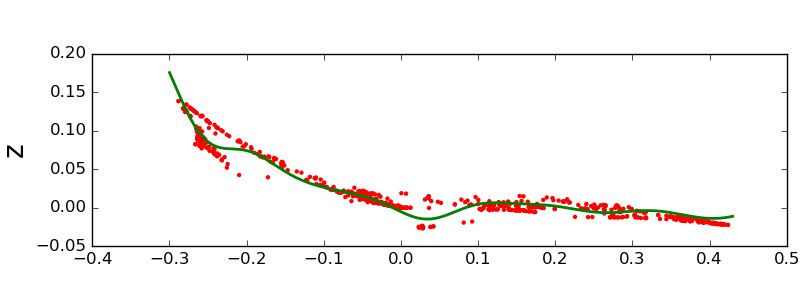
\includegraphics[width=0.9\textwidth]{ks22curveCoord}
    \\
    (b)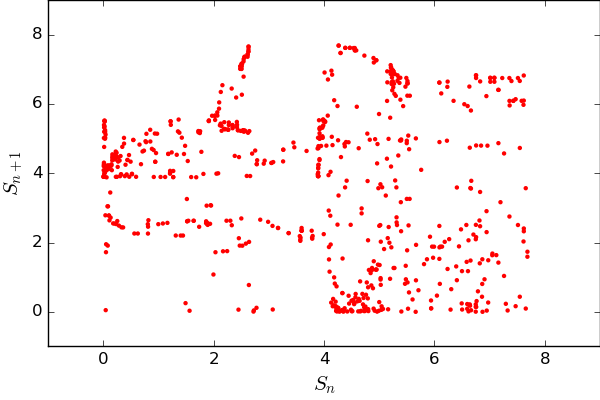
\includegraphics[width=0.9\textwidth]{ks22returnMap}
    \caption{
    \SFslice\ + invariant polynomial \refeq{XDD4reduc} reduction of \On{2}.
          (a) Regression curve ``fit'' (blue) of the
      {\PoincSec} \reffig{fig:ksPoinc}\,(d).
      (b) Return map.
    }
    \label{fig:ks22return}
  \end{figure}

\item[2016-05-23 Xiong]
  My previous figures are problematic because as the projection bases
  I used \EQV{2} eigenvectors
  which lie in invariant subspaces, with information lost
  in such projections. But still, I think \RPO{1} and the unstable
  manifold of \EQV{2} capture the essential dynamics of the system.
  I turn to the \fFslice\ $\Re(\hat{a}_1) = 0, \Im(\hat{a}_1) > 0$
  and use the reflection to transform trajectories into fundamental
  domain $\Re(\hat{a_2}) > 0$. \EQV{2} and \EQV{3} are in the {\sliceBord}, but
  the unstable manifold of \EQV{2} in the slice is unique, see
  Burak's argument in \emph{./ksRecycled/} draft
  (\HREF{../ksRecycled/tex/BuDiCv15.pdf}{click here})%
  \PC{
Burak writes: ``In this figure, $E_2$
and $E_3$ appear multiple times with extra subscripts ``u'' and ``s''
for a rather subtle reason: $E_2$ and $E_3$ are special solutions
which are symmetric under shifts by $L/2$ and $L/3$ respectively. In
other words, they respectively have non-zero components only at
multiples of second and third Fourier mode and no first mode
component. As a consequence, the
{\fFslice} % transformation \refeq{e-ffSliceSO2}
do not reduce the symmetry of these solutions;
they lie in the \sliceBord. However, some of their
linear stability eigenvectors (the ones which are relevant for generic
dynamics) do have different first Fourier mode components, and hence,
the corresponding stable and unstable manifolds have unique locations,
determined by the first Fourier mode phase of the respective stability
eigenvector, in the symmetry reduced \statesp. %\refeq{e-sspRefRed}.
''
  }.
  Still, I failed to  find a good basis set to project trajectories. I
  tried unstable eigenvectors of $\REQV{}{1}$, but the result is terrible.
  Again, I regressed to Fourier mode projection in order to obtain some
  feeling about the shadowing structure of the set of \rpo s.

\item[2016-04-23, 2016-05-25 Predrag]
I think your definition of the \reffig{fig:ks22return}\,(a) `regression
curve' is wrong. If you can define a 1\dmn\ segment of unstable manifold
we'll be in much better shape. You can see what is wrong with it by
looking at \reffig{fig:ksPoinc}\,(b): you are including into your
``regressive'' fit as nearby section points of trajectories which are
departing for very different parts of the attractor, \ie, they are far
away from each other in the \PoincSec\ (remember, L2-notion of distance
is nonsense, it counts as `close' points that sit on distinct folds of
the unstable manifolds - the correct distance is measured along the
unstable manifolds). For that reason you have multiple-valued return map
\reffig{fig:ks22return}\,(b). The good news is that you can see that
subsets of the return points do align themselves along lines, so if you
were more careful in defining the base segment of the {\PoincSec} by a
segment of an unstable manifold, they will align themselves into
identifiable return map folds.

Do that please first not for the 2nd Fourier mode slice, but for the
{\fFslice} in the \On{2} fundamental domain {\PoincSec} - figures you
have shown me on your computer screen.

\item[2016-05-25 Predrag]
Please, as a matter of course, always plot a square as a square (the same
units of length on the $x$- and $y$- coordinates in
\reffig{fig:ks22return}\,(b), though waste no time on this figure, that
is a remark for the future return maps).

\item[2016-05-23 Xiong]
  I'll try to have a look at the unstable manifold of $\REQV{}{1}$, which
  looks like a mess.

\item[2016-05-25 Predrag]
I do not think it makes sense to keep trying to focus on unstable
manifolds of \eqva\ and \reqva\ for now, with exception of \EQV{2}.

\item[2016-05-23 Xiong]
  \RPO{1} is frequently shadowed.

\item[2016-05-25 Predrag]
One of the most shadowed orbits seems to
be \RPO{1}, so use a periodic point $\ssp_0 \in {\PoincS}$ somewhere nice
along \RPO{1} in the fundamental domain (one of your computer screen
pictures), together with its Floquet vectors to define a \PoincSec\
${\PoincS}$, and trace out its unstable manifold in {\PoincS}, up to the
first turnback. A few forward iterates of that unstable manifold should
teach what \po s $ \in \pSRed$ (some are in \reftab{tab:ksShadow}) belong
to the local return map of \RPO{1} horseshoe.

In particular, look carefully at \reffig{fig:ksPoinc}\,(b), and note the
prominent family of orbits in the lower-left quadrant, shadowing \RPO{1}
(not drawn). They presumably form a repelling or (according to Burak)
nearly repelling horseshoe, not visible in the natural, ergodic density
plot \reffig{fig:ksPoinc}\,(a). Their local \PoincSec\ is the first
candidate for obtaining clean return maps and symbolic dynamics for a
subset of the symmetry-reduced \statesp\ \po s.

%%%%%%%%%%%%%%%%%%%%%%%%%%%%%%%%%%%%%%%%%%%%%%%%%%%%%%%%%%%%%%%%%%%%%%
\begin{figure} %[h]
  \centering
  (a)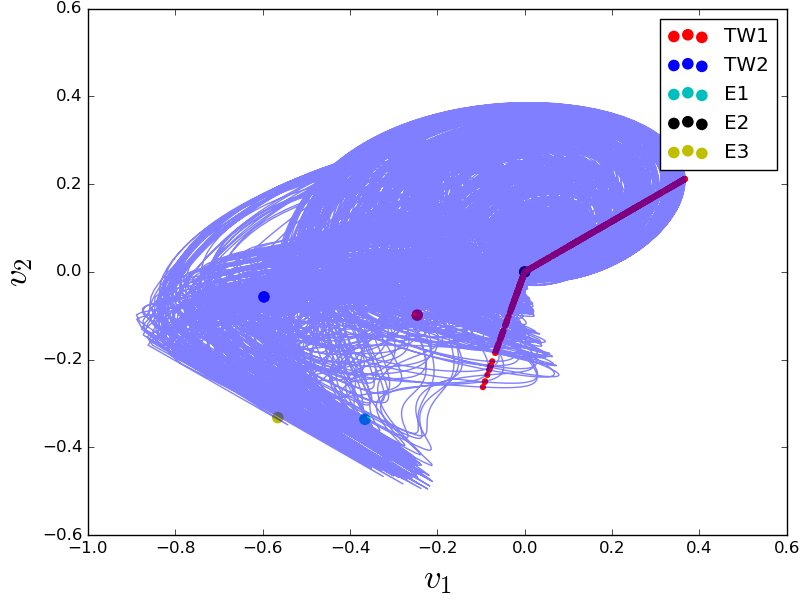
\includegraphics[width=0.46\textwidth]{ksPoinc}
  (b)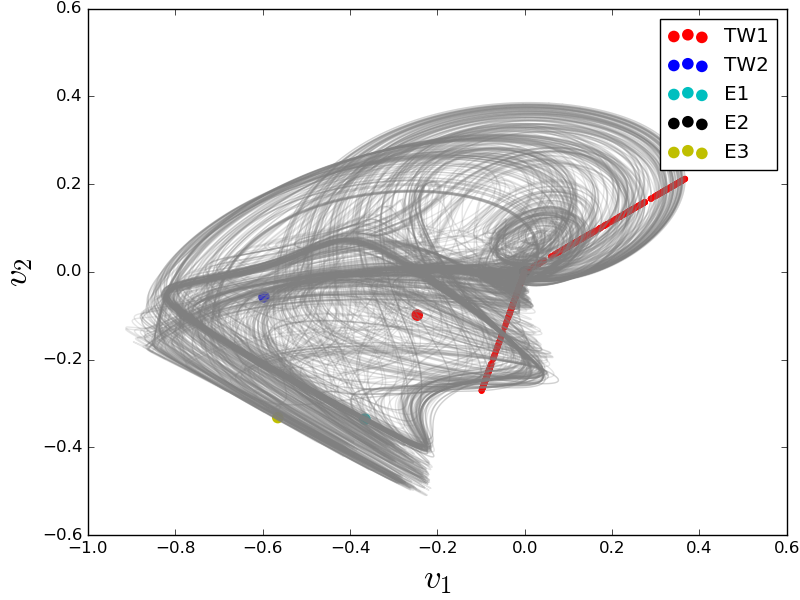
\includegraphics[width=0.46\textwidth]{ksPoPoinc}
  (c)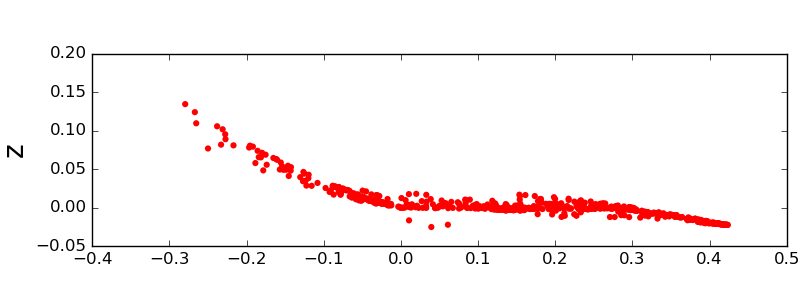
\includegraphics[width=0.46\textwidth]{ksPoinc2}
  (d)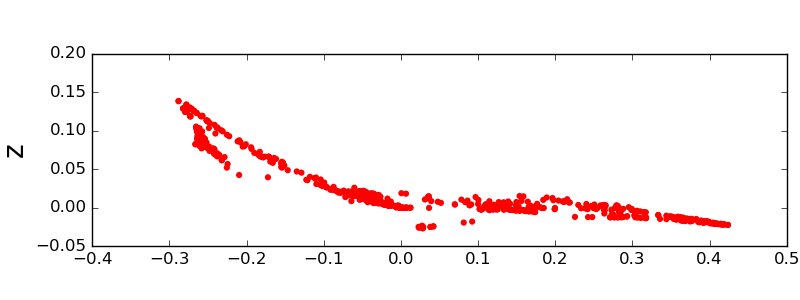
\includegraphics[width=0.46\textwidth]{ksPoPoinc2}
  \caption{
    \SFslice\ + invariant polynomial \refeq{XDD4reduc} reduction of \On{2}.
    (a) A long ergodic trajectory and the \PoincSec\ points
    (red).
    (b) The first 100 \ppo s and 100 \rpo s (gray) with the \PoincSec\
    points (red). Note the prominent family of orbits in the lower-left
    quadrant, shadowing
    \RPO{1} (not drawn). They presumably form a repelling or (according
    to Burak) nearly repelling horseshoe, not visible in the natural, ergodic
    density plot (a). Their local \PoincSec\ is the first candidate
    for obtaining clean return maps and symbolic dynamics for a
    subset of symmetry-reduced \statesp\ \po s.
    (c) \PoincSec\ points, ergodic trajectory (a).
    (d) \PoincSec\ points, 200 orbits (b).
  }
  \label{fig:ksPoinc}
\end{figure}
%%%%%%%%%%%%%%%%%%%%%%%%%%%%%%%%%%%%%%%%%%%%%%%%%%%%%%%%%%%%%%%%%%%%%%%

\item[2016-05-23 Xiong]
  There are quite a few nearby \rpo\ pairs, like \\
  (\RPO{5}, \RPO{6}),
  (\RPO{22}, \RPO{25}), and (\RPO{29}, \RPO{30}).

  \RPO{17} and \RPO{18} are not a pair, but actually the same orbit.
  My source file has some error. Predrag has told me for several times
  that these pairs are the consequence of the fact that the
  domain size is slightly larger than the bifurcation point. I do not
  know how to verify it.

\item[2016-05-25 Predrag]
  We'll return to \RPO{17} and \RPO{18} once return maps for other orbits
  are working.

\item[2016-05-23 Xiong]
  So far, I have not had a look at \ppo s.

\item[2016-05-25 Predrag]
  It will be worth looking at them soon, to fill out your return (or
  map-forward) maps. They tend to shadow \rpo s for reasons that I have
  never understood.

\item[2016-05-23 Xiong]
  What concerns me is \RPO{26}. Its shadowing behavior is quite different
  from that of \RPO{20} to \RPO{30}, because it only shadows \RPO{1}. So
  if I cut off the part of \RPO{26} that shadows \RPO{1}, I should obtain
  a trajectory showing a short \rpo\ or the unstable manifold of \EQV{2}. But
  the trajectory clearly shows that it does not shadow unstable manifold
  of \EQV{2}, nor any shorter \rpo. Maybe there is a new shorter orbit, or it
  is shadowing another invariant structure.

\item[2016-05-25 Predrag]
  Let's look at \RPO{26} later, after the horseshoe for the \RPO{1}
  family has been worked out.

\item[2016-05-25 Xiong] (Google chat entered here by Xiong's trusty secretary)
My (secret,  nowhere described) projection has problem because of the
discontinuity of trajectories in the fundamental domain. They look like
scattered pieces after the $\Zn{2}$-reduction.

\item[2016-05-31 Predrag]
Of course they look like scattered pieces after projection: they
\emph{have to} look like discontinuous trajectory segments after the
$\Zn{2}$-reduction. It's the same, except more complicated, for the
$\Dn{3}$-symmetric 3-disk pinball - that's why I wrote so much about it in
ChaosBook - maybe reread that? Like here, every reflection leads to a
discontinuity in the phase-space trajectory, and no matter what
projection you use, the trajectories in the $\Dn{3}$-reduced phase-space
are an unintelligible mess.

However, we could use experience with $N$-disk pinballs to tell us what
to do here. There there were 2 natural \PoincSec s; the boundary of the
disk (there is only one in the $\Dn{3}$-reduced phase-space), or the
symmetry axis for the reflection.

So why don't you try the reflection hyperplane (\ie, the fundamental
domain border in the {\fFslice}), invariant under the reflection
\refeq{BB1stSlRefl} and use it as a \PoincSec, and than look at it in any
of many ways you have available (I would prefer to have it centered on
\RPO{1}, as explained at length above). We might miss some \rpo s, but we'll
return to that later. All \eqva\ are in this \PoincSec, but not \reqva.
%(I believe, but not sure about that).

And remember, you should report your work in the blog - as long as it is
only on your screen there is no way Burak and I can give you constructive
input. For example, can you write down here why your
\reffig{fig:ks22return}\,(a) is \underline{wrong}? Or respond to my
comment by saying that you do not understand it, so that we can discuss
it in an online conversation?

Please put this project as \#~2 at the top of your stack (\#1~1 is
resubmitting the PR Lett), we have to make progress on this sooner rather
than later.

\item[2016-05-31 Xiong]
I have upload configurations of the 50 shortest \rpo s (like
\reffig{fig:rpo1522a}) in folder \texttt{figs/KSshadow}. They should help
us develop some intuition about the shadowing structure.

\item[2016-05-31 Predrag]
I love these, thanks! Gold mine of orbits to play with. Would it be much
bother to also add the 50 shortest \ppo s? My impression is that they
pair up nicely with the \rpo s.

The problem with these figures is that you chose to ignore
discontinuities, so it is hard to see where the fundamental domain border
lies. \refFig{fig:rpo1522b}, or an honest projection (with all Fourier
components, and with the correct definition of the fundamental domain
border) would be more helpful to see where the \PoincSec\ lies.


\item[2016-05-31 Xiong]
%Predrag is right. I need suggestions desperately.
Why is eigenvector bases projection better than Fourier projection? \KS\ system
is not like two-mode system. Stability vectors/Floquet vectors shape dynamics
only locally, then it does not make sense to project to them globally.

\item[2016-05-31 Predrag]
We are not interested in tracking continuous trajectories, we only need
to visualize a well-chosen \PoincSec, or a small set of \PoincSec s.
These could be rather local - the strange set was generated by sequences
of bifurcations from simple, initially stable limit cycles, and
the strange set \emph{in the \PoincSec} might be well captured by the
transverse tangent space at a point of a \po\ in its center.

The problem with not being able to liberate oneself from the 1990's
outmoded individual Fourier modes as projection axes is nicely
illustrated by \reffig{fig:rpo1522a}: \emph{every} orbit, represented by
its full Fourier series, is discontinuous if it crosses the fundamental
domain border, but if you use very special axes, like $\Im(a_j)$, it
\emph{appears} continuous. So do not use these silly Fourier mode axes -
it is a bad habit, and they will be increasingly more misleading as you
look at larger $L$ domains.

%%%%%%%%%%%%%%%%%%%%%%%%%%%%%%%%%%%%%%%%%%%%%%%%%%%%%%%%%%%%%%%%%
\begin{figure} %[h]
  \centering
  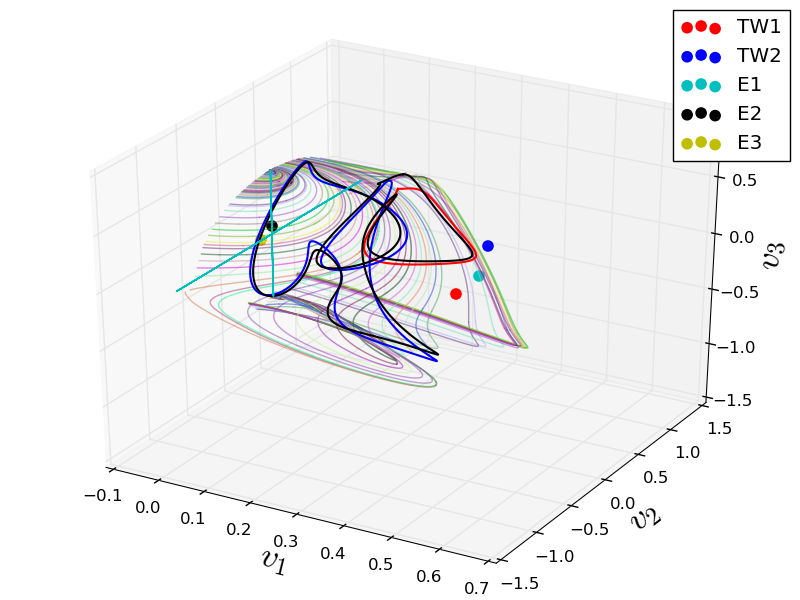
\includegraphics[width=0.99\textwidth]{rpo1rpo5rpo22Im}
  \caption{
    \SFslice\ + invariant polynomial \refeq{XDD4reduc} reduction of \On{2}.
    \RPO{22}, its shadowing orbit pair \RPO{1}+\RPO{5} (see
    \reftab{tab:ksShadow}), and the unstable manifold of \EQV{2} in the
    fundamental domain projected on raw Fourier components. (red) \RPO{1},
    (blue) \RPO{5} and (black) \RPO{22}. The dense set of gray curves is in
    the unstable manifold of \EQV{2}. The two green straight lines are the
    group orbits of \EQV{2} and \EQV{3} respectively.
        \PCedit{ % 2016-05-31
    Projection axes are the imaginary parts of the first 3 Fourier modes
    $[v_1, v_2, v_3] = [c_1, c_3, c_2]$, \ie, this is invariant under
    reflection in the full \statesp, and in the Xiong's {\fFslice}
    \refeq{XDinsliceRefl}. Note: were {\fFslice} Burak's, according to
    \refeq{BudCvi15-EvenOdd}, these modes are  not reflection invariant
    in the {\fFslice}. In a generic projection of the fundamental
    domain all orbits are discontinuous.
                }
  }
  \label{fig:rpo1522a}
\end{figure}
%%%%%%%%%%%%%%%%%%%%%%%%%%%%%%%%%%%%%%%%%%%%%%%%%%%%%%%%%%%%%%%%%%


\item[2016-05-31 Xiong]
I do not think
fundamental domain border is a good candidate for \PoincSec.
\refFig{fig:rpo1522a} shows 3 \rpo s projected into different Fourier subspaces.
Here the leading 4 Fourier modes are all used, so I think these two figures
faithfully represent the dynamics. \refFig{fig:rpo1522a} is a projection onto a subspace
of the invariant anti-symmetric subspace (imaginary part of Fourier modes). The
shadowing is obvious. But this figure cannot tell us the jumps in the orbits,
because refection only flips the sign of real part of Fourier modes.

\refFig{fig:rpo1522b} shows
that there are two jumps in \RPO{1} (red curve). So if we chose the fundamental
domain border as the \PoincSec, then \RPO{1} is represented by 2 points on
it.


\item[2016-05-31 Predrag]
That is perhaps as it should be: \PoincSec\ is defined by the section
hypersurface, and the orientation of the crossing. You should really indicate
the direction on all these segments; in any case \RPO{1} (red)
seems to cross twice. Bummer - would be nicer if short \po s were
single fixed points on the section, not pairs of points.

Good news is that they shadow nicely, segment by segment.

\item[2016-05-31 Xiong]
Look at \RPO{22} (black curve), it does not jump at the place where \RPO{1}
jumps. Then in the \PoincSec, these two orbits (more precisely, two sets
of \PoincSec\ points) are far away, such that we are misled to ignore their
shadowing structure.

\item[2016-05-31 Predrag]
\RPO{22} shadows one short orbit, then shadows neither, then shadows the
other short orbit. If the \PoincSec\ happens to cut the in-between
segment of one particular shadowing orbit, it's OK. By the time you have
unstable manifolds under control and longer orbits, I think shadowing
will be clear.

\item[2016-05-31 Xiong]
Also, I choose the fundamental domain as $Re(a_2) > 0$, only because
$a_2$ is the next Fourier mode after $a_1$. But nobody says it will work.
The choice of fundamental domain in the 3 billiard system is based on
geometry: the border is perpendicular to the line connecting centers. If
not, the result will be terrible. Even center to center bouncing is hard
to tell. However, I do not have enough intuition in \KS.

\item[2016-05-31 Predrag]
Read my concrete proposal for how to define the fundamental domain...

%%%%%%%%%%%%%%%%%%%%%%%%%%%%%%%%%%%%%%%%%%%%%%%%%%%%%%%%%%%%%%%%%
\begin{figure} %[h]
  \centering
  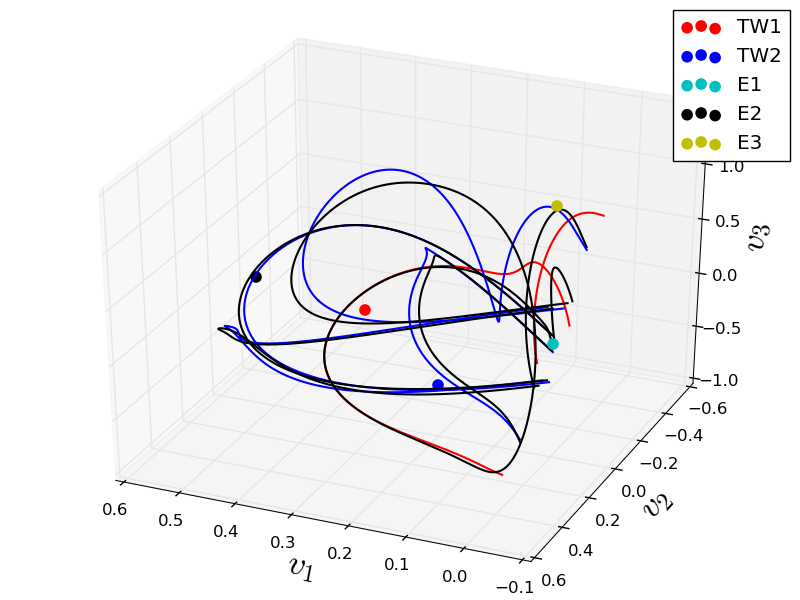
\includegraphics[width=0.99\textwidth]{rpo1rpo5rpo22Re}
  \caption{
    \SFslice\ + invariant polynomial \refeq{XDD4reduc} reduction of \On{2}.
    The same orbits as in \reffig{fig:rpo1522a}: (red) \RPO{1}, (blue)
    \RPO{5} and (black) \RPO{22}, projected on the real Fourier modes
    $[v_1, v_2, v_3] = [b_2, b_4, b_3]$. The group orbits of \EQV{2} and
    \EQV{3} are not displayed.
    The unstable manifold of \EQV{2} disappears because it is in the
    antisymmetric invariant subspace $\bbU^+$ \reftab{tab:EksymE2} for which,
    by definition, $b_i = 0$.
  }
  \label{fig:rpo1522b}
\end{figure}
%%%%%%%%%%%%%%%%%%%%%%%%%%%%%%%%%%%%%%%%%%%%%%%%%%%%%%%%%%%%%%%%%%


\item[2016-05-31 Predrag]
You seem to be using the full-state space definition of the reflection
operation. The correct definition of the reflection in the {\fFslice}  is
\refeq{BB1stSlRefl}, or, in the real representation\rf{BudCvi15},
the action of the reflection on the slice coordinates is
\bea
&\matrixRepRed (\Refl)& (\hat{b}_2, \hat{c}_3, \hat{b}_4,
\hat{c}_5, \hat{b}_6, \hat{c}_7, \ldots )
\continue
&& = (-\hat{b}_2, -\hat{c}_3, -\hat{b}_4,
-\hat{c}_5, -\hat{b}_6, -\hat{c}_7, \ldots )
\,,
\label{BudCvi15-EvenOdd}
\eea
where we for brevity omit all terms whose signs do not change under
reflection.

The fundamental domain border is not a codimension-1 hyperplane;
if the dimension of the full \statesp\ is $2N$, its dimension is
approximately $N$ (please do the correct counting). So the normal
to the border
\beq
(\hat{b}_1, 0,0,\hat{c}_2, \hat{b}_3,0,0,
\hat{c}_4, \hat{b}_5, 0,0,\hat{c}_6, \ldots )
\ee{PCfundBorder}
is not a vector, but ``$N$''\dmn\ normal hyperplane
\beq
(0,0,\hat{b}_2, 0,0,\hat{c}_3, \hat{b}_4,0,0
\hat{c}_5, \hat{b}_6, 0,0,\hat{c}_7, \ldots )
\ee{PCfundNormal}

The (perhaps?) simplest fundamental domain border \PoincSec\ codimension-1
hyperplane can thus
 be defined by
\beq
\hat{n} = (0,0,1,0,0,0,\ldots )
\ee{fFsliceFundDomPSec}


%%%%%%%%%%%%%%%%%%%%%%%%%%%%%%%%%%%%%%%%%%%%%%%%%%%%%%%%%%%%%%%%%%
A {\template} and the associated hyperplane Poincar\'e section
(excerpted from ChaosBook Example~3.1):

The simplest choice of a Poincar\'e section is a plane $\PoincS$
specified by a `\template' point (located at the tip of the vector
$\slicep$) and a normal vector $\hat{n}$ perpendicular to the plane. A
point $\sspRed$ is in this plane if it satisfies the linear condition
\beq
    \PoincC(\sspRed) = (\sspRed-\slicep) \cdot \hat{n} = 0
    \qquad \mbox{for } \sspRed \in \PoincS
\,.
\ee{PSPlane}
Consider a short periodic orbit roughly centered at $\slicep$, but not lying
in $\PoincS$. It pierces the hyperplane twice; the $\vel \cdot \hat{n}  >
0$ traversal orientation condition ensures that the
first return time is the full period of the cycle.
%%%%%%%%%%%%%%%%%%%%%%%%%%%%%%%%%%%%%%%%%%%%%%%%%%%%%%%%%%%%%%%%%%

\item[2016-05-31 Predrag]
Proposal:
{\bf A fundamental domain border \PoincSec:}
Mark on every \rpo, \ppo\ and ergodic trajectory
by fat points the instants where
\(
\sspRed_p(\zeit)\cdot \hat{n} = 0
\)
and
\(
\vel(\zeit) \cdot \hat{n}  >
0
\)

\item[2016-06-02 Xiong] I added the shortest 50 \ppo s in folder
\texttt{figs/KSshadow/}. A lot of shadowing instances between \ppo s and
\rpo s can be identified.

\item[2016-06-02 Xiong] A clarification about the
definition of the fundamental domain in my \fFslice.

I am using \fFslice\ condition $b_1 = 0, c_1>0$, so orbits are rotated
to the imaginary axis of the 1st mode. The benefit of doing this
is that it keeps the reflection law $a_k \to -a_k^*$ unchanged
in the slice.

\item[2016-06-03 Predrag]
That's nice!

\item[2016-06-06 Ruslan] I'm happy to see that you are now
thinking about the fundamental domain along the same lines I did
over 8 years ago.  Unfortunately, I never found enough time since then to
continue developing these ideas.  I hope Xiong will be more successful.
You might find it useful to review my notes on this in
{\tt blog/davidchack/071231fundamental.html}.

\item[2016-06-02 Xiong]
Suppose 2 points in the full state space are
the reflection of each other: $x_2 = \Refl x_1$, then one needs $\theta$
and the other needs $-\theta$ to rotate onto slice:
$\hat{x}_1 =g(\theta)x_1$, $\hat{x}_2 =g(-\theta)x_2$. Therefore,
$\hat{x}_2 =g(-\theta)\Refl x_1 = \Refl g(\theta)x_1 = \Refl\hat{x}_1$. So
reflection does not change form in slice, and the law in
\refeq{BudCvi15-EvenOdd} should be replaced by
\beq
  (0, \hat{c}_1 , \hat{b}_2 , \hat{c}_2 , \hat{b}_3 ,\hat{c}_3 ,\cdots)
  \to
  (0, \hat{c}_1 , -\hat{b}_2 , \hat{c}_2 , -\hat{b}_3 ,\hat{c}_3 ,\cdots)
\ee{XDinsliceRefl}
Namely, $b_k = \Re(a_k)$ changes sign. So the general choice of fundamental
domain is a linear combination of $b_k$'s:
\begin{equation}
  \label{eq:ksfundDomain}
  U(b_k, c_k) = \sum_{k=2}\alpha_k b_k >0 \,.
\end{equation}

This is analogous to the Lorenz case : $(x, y, z)\to (-x,-y, z)$.
Look at $x-z$ or $y-z$ plane, it is reflection, the fundamental
domain is $x>0$ or $y>0$ respectively. Look at the $x-y$ plane,
it is $C_2$ and fundamental domain is $\alpha_1 x + \alpha_2 y >0$
in \KSe\ slice.

\item[2016-06-03 Predrag]
Cannot be analogous to the Lorenz case; that is a symmetry
under rotation by $\pi$, so any radial half-plane can serve
as a fundamental domain border. For \KS\ in full \statesp\
the reflection hyperplane is fixed relative to real axis;
no rotation arbitrariness.

\item[2016-06-02 Xiong]
Also, as you suggested, if we choose the
fundamental domain border $\sum_{k=2}\alpha_k b_k =0$ as the
\PoincSec, then the template point is fixed at
$\hat{a}'= (0, 0,\cdots, 0)$
with direction $(0, 0, \alpha_2, 0, \alpha_3, 0, \cdots)$. We could not
choose $\hat{a}'$ freely.


\refFig{fig:ksfundPoinc} shows the
result of \PoincSec\ points by setting $\alpha_2 = 1$ and
all other $\alpha_k=0$. The 200 orbits used here intersect this
\PoincSec\ at most 7 times each. The scattering plot shows some thin
structure, but it does not look any better than
\reffig{f-psect_eq2tw1_400rpoppo}.

\item[2016-06-03 Predrag]
Maybe. But it looks vastly better than \reffig{fig:ksPoinc}\,(c), and
(d), as now most of the periodic points lie on distinct smooth 1D curves.

However, are you sure that your \PoincSec\ is defined by the section
hypersurface, \emph{and the orientation of the crossing}? Are short \po s
are single fixed points of the section, not pairs of points? Also, as in
general every orbit is discontinuous after reflection into the
fundamental domain, you have to decide whether you are plotting the point
at time $\epsilon$ before the reflection, or after the reflection.

\item[2016-06-02 Xiong] I am worried about constructing a wrong
\PoincSec\ before I building enough intuition about the geometric
structure of the attractor.
\begin{figure} %[h]
  \centering
  (a)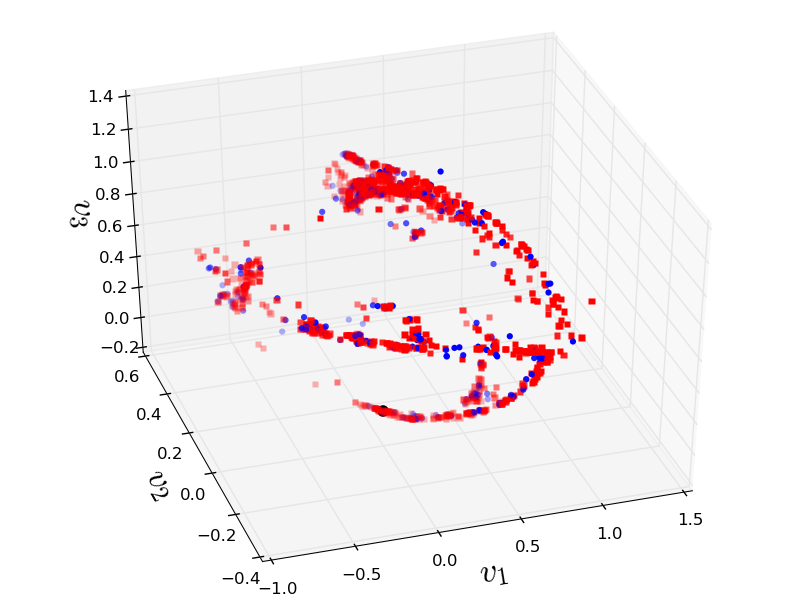
\includegraphics[width=0.6\textwidth]{KSPoPoincare}
  (b)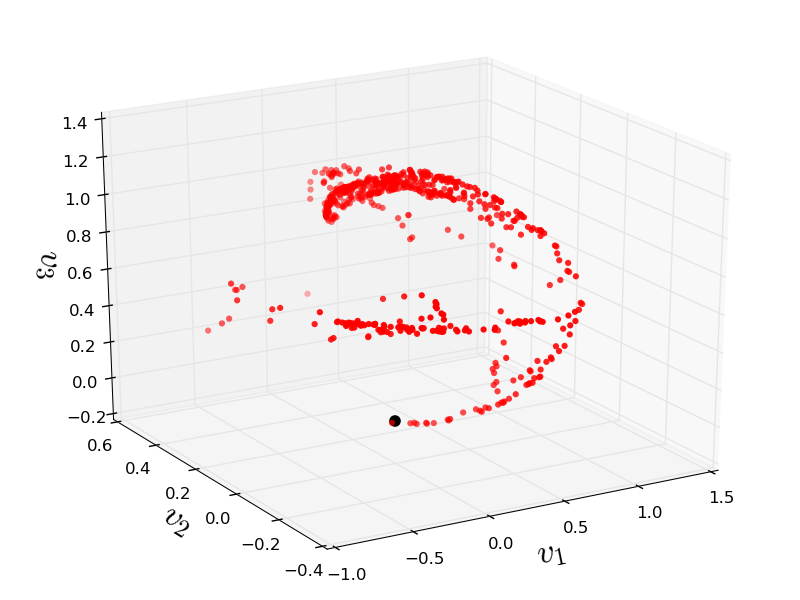
\includegraphics[width=0.6\textwidth]{KSErgodicPoincare}
  (c)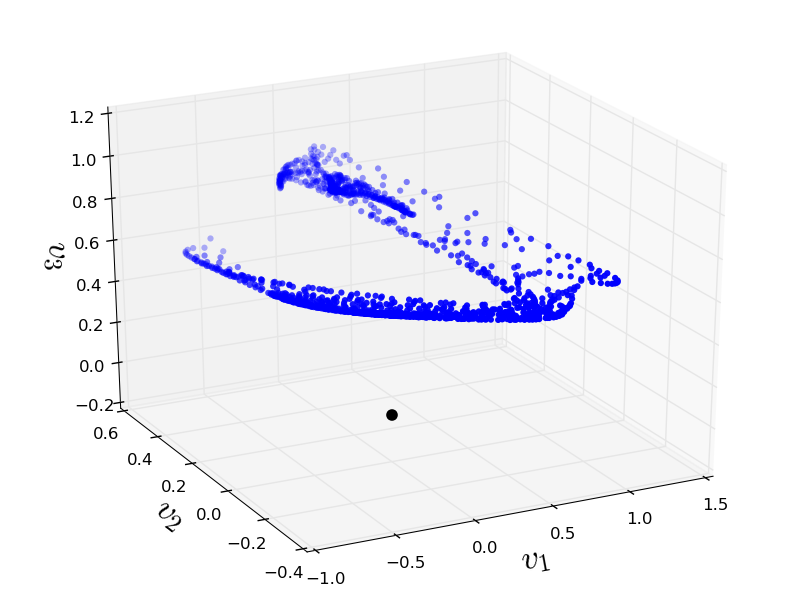
\includegraphics[width=0.6\textwidth]{KSE2Poincare}
  \caption{
    \SFslice\ + invariant polynomial \refeq{XDD4reduc} reduction of \On{2}.
    A \PoincSec\ of the \KS\ flow, with \On{2} symmetry quotiented out,
    projected from a 62\dmn\ full \statesp\ flow down to 3 dimensions.
    The black point is the \PoincSec\ point
    of \RPO{1}, taken as the the origin of the plots.
    (a) \PoincSec\ points of the shortest 100 \rpo s (red circles)
    and shortest 100 \ppo s (blue squares).
    (b) \PoincSec\ points of an ergodic trajectory.
    (c) \PoincSec\ of the unstable manifold of \EQV{2}.
    The three sets can be viewed together
    \HREF{http://www.cns.gatech.edu/~xiong/figs/mixPoincare.html}
    {here}:
      (red) ergodic trajectory \PoincSec\ points;
      (green) \PoincSec\ periodic points, 200 prime \po s;
      (blue)  \PoincSec\ of the \EQV{2} unstable manifold.
  }
  \label{fig:ksfundPoinc}
\end{figure}

\item[2016-06-03 Xiong]
I think \refeq{eq:ksfundDomain} is the reflection hyperplane. Reflection
flips $b_k$, so $\Refl U(b_k, c_k)= -U(b_k, c_k)$. So, this is really analogous
to Lorenz system.

I have updated \reffig{fig:ksfundPoinc}. Here, \PoincSec\ does not change:
$\hat{b}_2 = 0$ with direction from negative to positive, and I only
take the point immediately after it crosses \PoincSec. So they are
actually not exactly on the \PoincSec, but very close to it and they
are in the fundamental domain. \RPO{1} has only one \PoincSec\ point.
I use its one unstable and two least stable
in-slice Floquet vectors to construct 3 orthonormal bases.
\refFig{fig:ksfundPoinc} are projection to these bases with this point
as origin. The scatter in these plots is not easy to visualize, so I provide
some interactive plots online for you to have a better feeling (try to
rotate these figures).
The \PoincSec\ of unstable manifold of \EQV{2} looks good, but it is in
the invariant subspace. To me, the \po s \PoincSec\ points look terrible.

\item[2016-06-04 Predrag]
That's funny - \reffig{fig:ksfundPoinc}\,(a) now looks worse. The online
3D plots are wonderful! This \PoincSec\ confirms Burak's results - the
strange set is surprisingly thin, I'm very hopeful about chances that we
can partition it and get some reasonable return (or forward) \Poincare\
maps.

\item[2016-06-04 Predrag]
I do not know how big the integration time-step
is, \ie, I do not have sense for how accurate your \PoincSec\ points are
compared to the size of your red dots. If they are more accurate than the
dot size, then it would be interesting to run
\reffig{fig:ksfundPoinc}\,(b) for much longer time, with much smaller
\PoincSec\ dots - that might reveal some fine structure of the unstable
manifold (\ie, the strange attractor). If \PoincSec\ points are
inaccurate (let's say more than 1 \%\ of the overall plot size), do not
bother, because the numerical noise will wipe out all fine structure.

\item[2016-06-06 Xiong] \PoincSec\ is $\hat{b}_2 = 0$. The data of
\PoincSec\ points has $\hat{b}_2$ in range $10^{-4}\sim 10^{-2}$. Few
of them will reach $10^{-1}$. The average magnitude of $\hat{b}_2$
in the slice has order about $10^{-1}$. So the \PoincSec\ points are
not too accurate.

\item[2016-06-04 Predrag]
I think I was wrong to claim that ``{\bf 2016-05-25 Predrag} One of the
most shadowed orbits seems to be \RPO{1}.'' \RPO{1} / \PPO{2} pair is
shadowed by some longer orbits, in striking ways, but is rarely visited
by the ergodic orbit: in \reffig{fig:ksfundPoinc}\,(b) there seems to be
a hint of the \RPO{1} unstable manifold, but natural measure is rather
far away from the origin (the \RPO{1} fixed point in the \PoincSec).
Also, while most of the measure seems to be in a plane, the \RPO{1}
unstable manifold is in a different plane transverse to it (in these 3
coordinates). So maybe there will be some local \PoincSec\ we will
need to describe its neighborhood, but that will not be the most
important \PoincSec.

\item[2016-06-04 Predrag]
The unstable manifold of \EQV{2} \reffig{fig:ksfundPoinc}\,(c) seems to have
little, if anything, to do with the strange attractor...

Can you plot the group orbit of \EQV{2}, or the point on it where \EQV{2} is
closest to its unstable manifold? Currently \EQV{2} and its unstable manifold
look disconnected...

\item[2016-06-06 Xiong]
I made some mistake in obtaining \PoincSec\ points of unstable
manifold of \EQV{2}. It is in the invariant subspace
$\hat{b}_k=0$, so the entire manifold should be in the \PoincSec. Initially,
I used the same method for \po s and ergodic trajectory to get \PoincSec\ points
of unstable manifold of \EQV{2}, which is wrong.
\refFig{fig:ksfundPoinc} is updated with a link pointing to a plot showing
all 3 cases in the same frame.

\item[2016-05-23 Xiong]
  \refTab{tab:ksShadow} shows whether the shortest 30 \rpo s are shadowing
  the unstable manifold of \EQV{2} or some shorter \rpo s. My observations
  are tentative.

  \begin{table}
    \centering
    \begin{tabular}{l | l | l | l}
      rpo & $T$ & shadow & $\sum T_i$ \\
      \hline
      1 & 16.31  & & \\
      2 & 32.80  & & \reffig{ks22rposMF}, \reffig{f:KS22rpo}:
                     the least unstable short \rpo\\
      3 & 33.50  & \EQV{2} & \\
      4 & 34.64  & & \\
      5 & 35.97  & & \\
      6 & 36.22  & \RPO{5} & \\
      7 & 39.70  & & \\
      8 & 40.14  & & \\
      9 & 41.50  & \EQV{2} & \\
      10 & 44.71  & & \\
      11 & 45.50  & & \\
      12 & 46.06  & & \\
      13 & 46.51  & \RPO{12} & 46.06\\
      14 & 47.32  & & \\
      15 & 47.64  & \EQV{2} & \\
      16 & 52.65  & \RPO{1}+\RPO{8}& 56.46 \\
      17 & 53.59  & \EQV{2} & \\
      18 & --.--  & same as 17 & \\
      19 & 54.76  & & \\
      20 & 55.60  & \EQV{2} & \\
      21 & 57.15  & \RPO{1}+\EQV{2} & \\
      22 & 57.59  & \RPO{1}+\RPO{5} & 52.28\\
      23 & 58.08  & \RPO{1}+\RPO{8} & 56.46\\
      24 & 58.11  & \RPO{1}+\EQV{2} & \\
      25 & 59.02  & \RPO{1}+\RPO{5} & 52.28\\
      26 & 59.64  & \RPO{1} & \\
      27 & 59.90  & \EQV{2} & \\
      28 & 62.96  & \RPO{26} & 59.64 \\
      29 & 63.20  & \RPO{1}+\RPO{12} & 62.38 \\
      30 & 63.70  & \RPO{1}+\RPO{12} & 62.38 \\
      $\RPO{64.51}$ & 64.51 & \RPO{1}+\RPO{14} & $01$, see \reffig{f:rpo_shad} \\
      $\RPO{80.71}$ & 80.71 & $\RPO{1}^2+\RPO{14}$ & $001$,  \reffig{f:rpo_shad} \\
    \end{tabular}
    \caption{
      \Rpo\ shadowing table. (\RPO{17} and \RPO{18} are the same solution,
      counted twice by error in Xiong's source file).
    }
    \label{tab:ksShadow}
  \end{table}

\item[2016-06-05 Predrag] Eyeballing orbits in folder
\texttt{figs/KSshadow/} separates them into bifurcation related quartets,
and suggests strongly that we might be missing some short orbits:

Shadowing the rarely visited  \RPO{1} / \PPO{2} or [rp1/pp2]:

\begin{verbatim}
[rp12/pp12 rp13/pp14]
rp16 /missing pp?/
pp16 /missing pp?/
[rp21/pp22/pp23 rp24/pp32]
[rp22/pp24 rp25/pp25]
rp23 /missing pp?/
[rp26/pp26 rp28/pp26]
[rp29/pp28 rp30/pp30]
[rp31/pp31 rp32/pp33]
rp43 /missing pp?/
rp45 /missing pp?/
[rp47/pp50]
\end{verbatim}

{\bf to Burak}: you wrote somewhere why \RPO{j} / \PPO{j} come in
pairs - where is that?

Embedded into denser regions of natural measure, presumably would like to
center \PoincSec\ on these:
\\
~[rp4/pp5 rp7/pp6]
\\
~[rp40/pp41 rp48/pp46]
\\
pp8 pp17 pp29 pp32 pp36 pp39 pp40  pp42 pp43 pp44 pp45

rp3/pp3  rp5/rp6 rp8/pp7 rp9/pp9 rp11/pp11 rp14/pp13 rp15/pp15

rp19/pp20

[rp20/pp21 rp21/pp22] rp22/pp24

[rp17/pp18 pp19] pp27/rp27 rp35/rp36 rp36/pp44

rp10 rp25 rp33/pp29 rp34/pp34 rp36 rp37 rp38 rp39  rp44

rp2 rp38 rp39

\item[2016-06-06 Ruslan] About missing short orbits: Of course I cannot
guarantee that there are no missing short orbits (the search was
extensive, but not systematically complete), but to me a more likely
scenario is that such orbits do not exist at $L = 22$, but might appear
at other values of $L$.  This would be similar to what we observe before
a Hopf bifurcation: we observe a near periodic dynamics, yet there are no
periodic orbits until we change a parameter past the bifurcation point.

\item[2016-06-06 Predrag] According to Burak, \ppo s are born first, than
come \rpo s through a symmetry breaking bifurcation. This bifurcation
must be described in the zillion applied math papers on \On{2}
bifurcations... That is consistent with your argument, as so far I'm
observing \ppo s without their \rpo\ cousins, not the other way around.

I'm a bit surprised that so many \ppo s have not yet bifurcated at $L=22$.
I would expect that $\Delta L$ for that bifurcation is small, especially
as the 1/2 the data set is \ppo s. In any case, it should be easy for us
to settle this by inspecting the  \ppo\ multipliers for the isolated
ones.

I am a bit intrigued that all of these come not in doublets, but in
quadruplets. Why?

And what about \rpo s that have not been born in bifurcations off \ppo s?
Shouldn't they also exist?

\item[2016-06-07 Burak] Another mechanism for the birth of \rpo s are
Hopf bifurcations of \reqva . For \KS\ at $L=22$, $TW_1$ has two
complex conjugate unstable eigenvalues but in my visualizations of
this manifold I could not find recurrent dynamics. However, I think it
is a good idea to continue $TW_1$ down in system size and
re-investigate this manifold. Because at
$L=22$, $\Re \lambda_{3,4} = 0.0337$ for $TW_1$, hence it's very close
to a bifurcation, if we eliminate that by going to a smaller system size
the remaining unstable manifold would be $2D$. So if there is a
\rpo\ born in this neighborhood, it would be much easier to find.

\newcommand{\primeOrb}[1]{\ensuremath{p_#1}}
\begin{figure}[h]
   	\centering
   	(a) 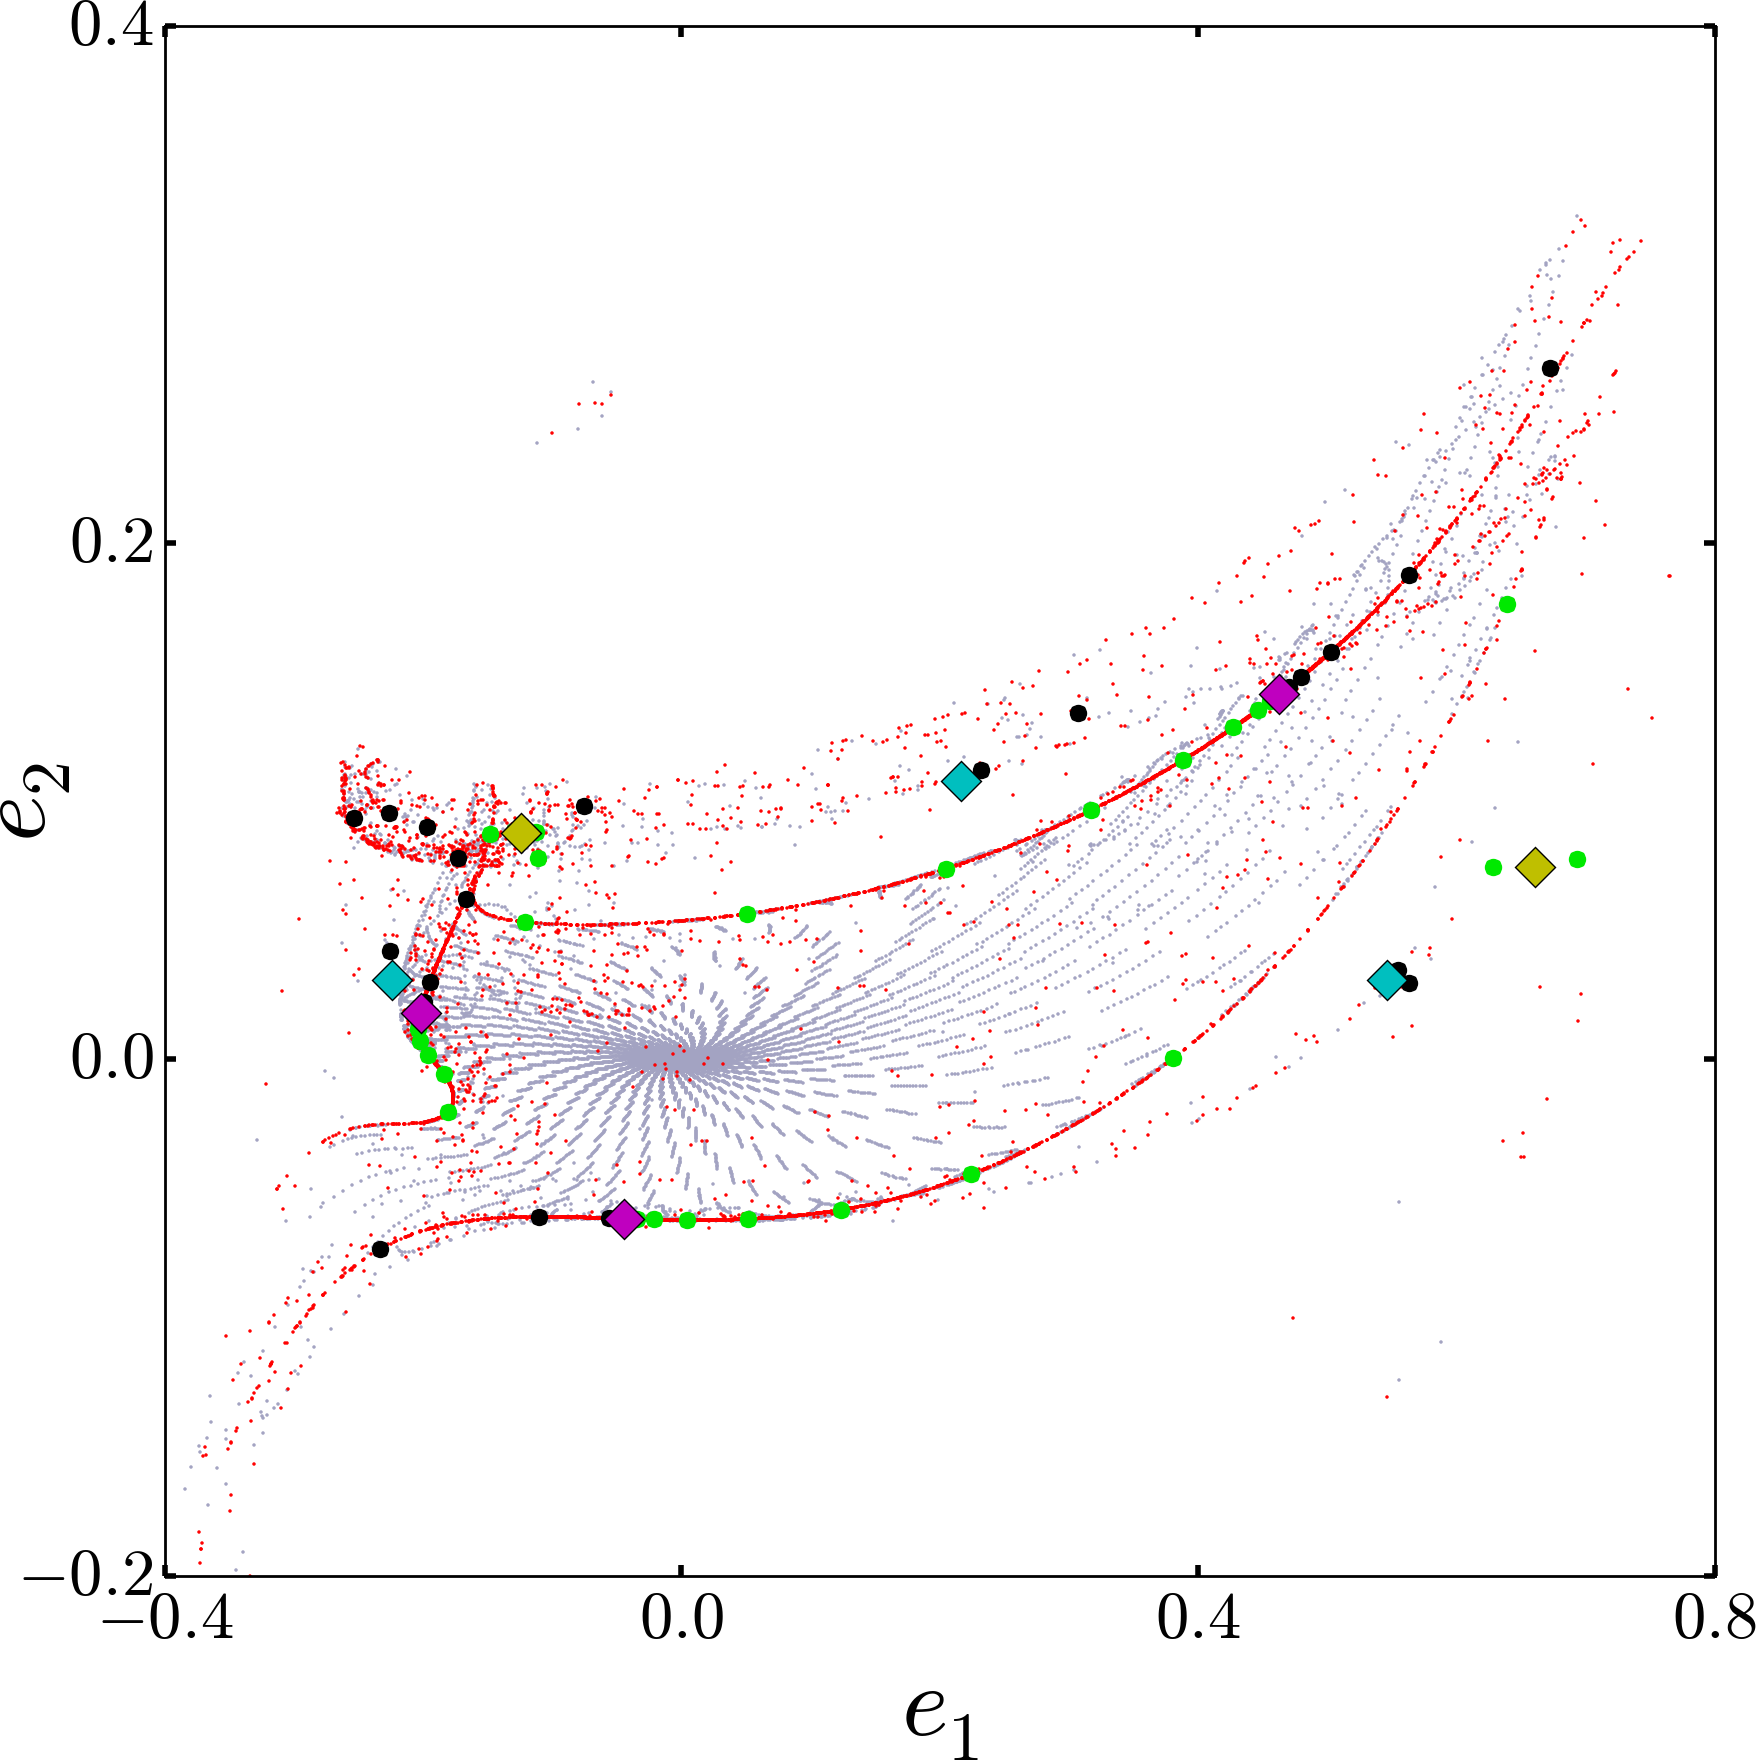
\includegraphics[height=0.40\textwidth]{UnstManPPO4L21p7png}
    (b) 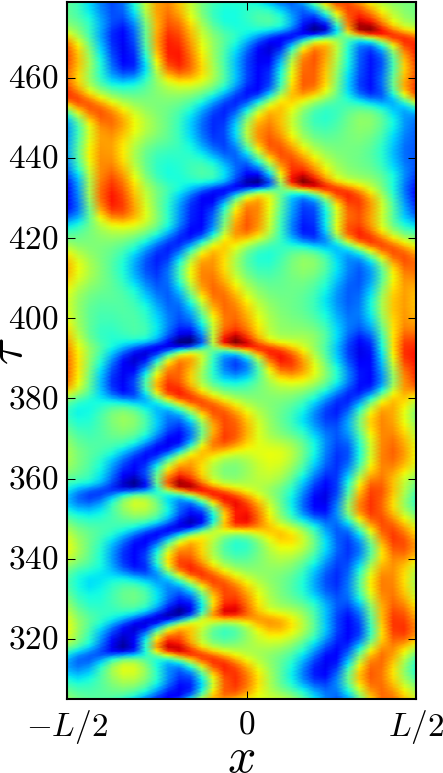
\includegraphics[height=0.40\textwidth]{KSHetCon21p7conf}
    (c) 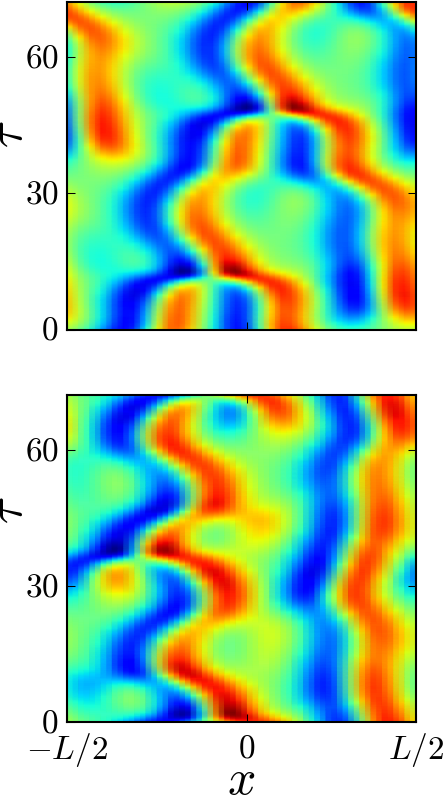
\includegraphics[height=0.40\textwidth]{KSHetCon21p7POsconf}
   		
   		\caption{\label{f-ConnectionsL21p7}
            (a) Unstable manifolds of $\primeOrb{0}$  (gray) and
   			\PPO{3} %$\primeOrb{1}$
            (red) on the Poincar\'e
   			section at $L=21.7$.
   			Magenta, cyan, and yellow diamond markers respectively show the
   			\PoincSec\ points of
            \PPO{3}, %$\primeOrb{1}$,
            $\primeOrb{3}$,
            and
   			$\primeOrb{4}$.
   			Green and black dots correspond to two individual orbits
   			started on the linear approximation to the unstable manifold
   			of \PPO{3}, %$\primeOrb{1}$,
            which visit neighborhoods of
   			$\primeOrb{3}$ and $\primeOrb{4}$ respectively.
   			(b) Space-time visualization of a segment of the orbit marked
   			green on (a) as it leaves the neighborhood of
            \PPO{3} %$\primeOrb{1}$
   			and enters the neighborhood of $\primeOrb{4}$.
   			(c) Space-time visualizations of
            \PPO{3} %$\primeOrb{1}$
            (bottom) and
   			$\primeOrb{4}$ (top).
   			From \refref{BudCvi15}.
   		}
\end{figure}

\item[2016-06-06 Burak] I copied \reffig{f-ConnectionsL21p7} from
\refref{BudCvi15} where I show appearance of an \RPO{}
on the unstable manifold of a \PPO{3}. This happens after \PPO{3}
undergoes a symmetry breaking bifurcation, \ie\  once it has a negative
real Floquet multiplier with absolute value greater than unity. The
Poincar\'e section of \reffig{f-ConnectionsL21p7} is around \PPO{1},
which has a $2D$ unstable manifold. I think this picture qualitatively
do not change at $L=22$; and I believe the natural next step from
\reffig{f-ConnectionsL21p7} is to compute unstable manifold of \PPO{3}
(referred to as $\primeOrb{1}$ in the caption) on its own local frame;
because in \reffig{f-ConnectionsL21p7} \PPO{3} appears in 3 locations
(it's period triple of \PPO{1}), so does its unstable manifold hence it
looks more complicated then it should. This is not so easy because
$2D$ the unstable manifold of \PPO{3} expands much faster in one
direction then the other, hence one needs a specially tailored
``locality'' condition for the Poincar\'e section that takes into
account for the shape of the manifold. It might be possible with some
continuity criterion.

In general, I think \PPO{} - \RPO{} pairs show up when \PPO{}s have
negative real unstable Floquet multipliers. These are the
symmetry-breaking instabilities and in the case of
\reffig{f-ConnectionsL21p7} it leads to the appearance of an \RPO{} of
similar period on the unstable manifold of the \PPO{}.

\item[2016-06-04 Predrag]
What other orbits are fixed points in the \PoincSec? Would be nice to
find one that is in the center of the natural measure (very roughly at
(0.5,0.4,0.4) in this projection).

\item[2016-06-06 Xiong]
Orbits \PPO{3}, \PPO{4}, \PPO{5}, \PPO{6}, \PPO{8} are fixed points
in \PoincSec, see  \reffig{fig:ppoFixedPts}.
\\
(this statement is wrong, see {\bf 2016-06-07 Xiong} below).

%%%%%%%%%%%%%%%%%%%%%%%%%%%%%%%%%%%%%%%%%%%%%%%%%%%%%%%%%%%%%%%%%%%%
\begin{figure}% [h]
\begin{center}
   \PPO{2} 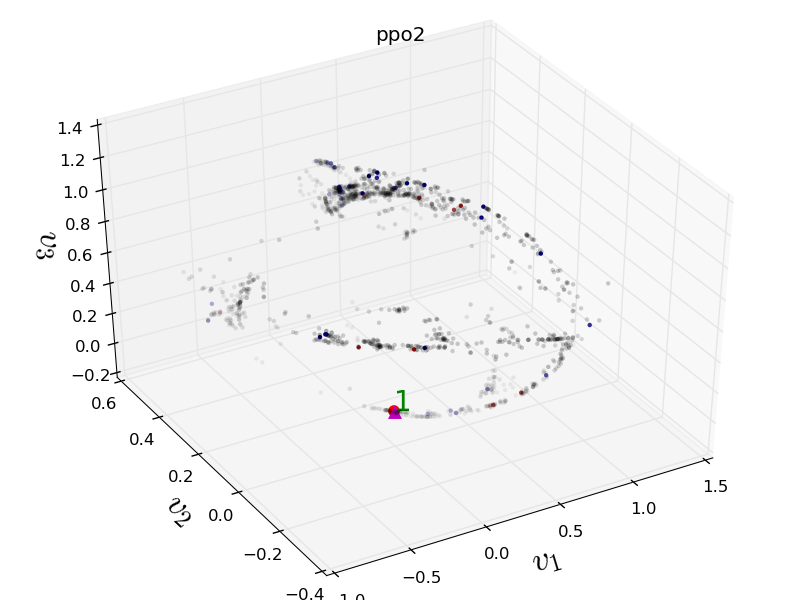
\includegraphics[width = 0.36\textwidth]{ppo2}
   \PPO{3} 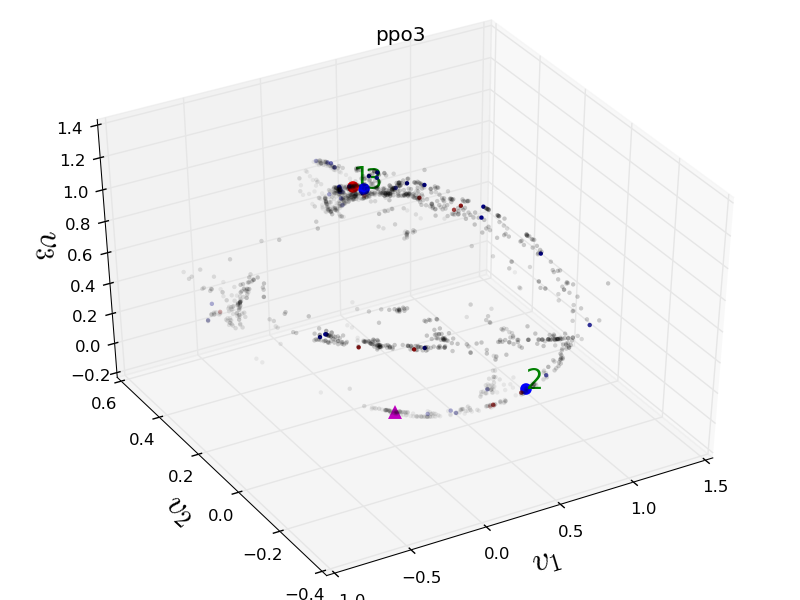
\includegraphics[width = 0.36\textwidth]{ppo3} \\
   \PPO{4} 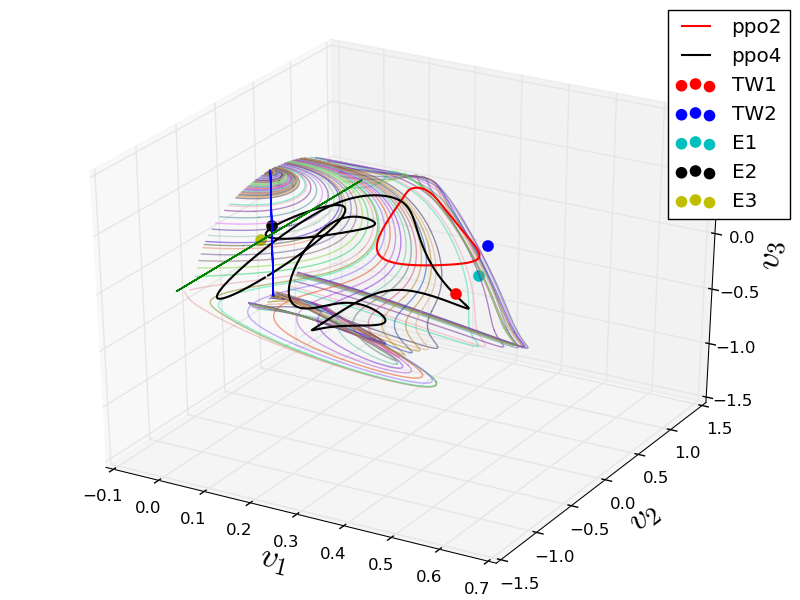
\includegraphics[width = 0.36\textwidth]{ppo4}
   \PPO{5} 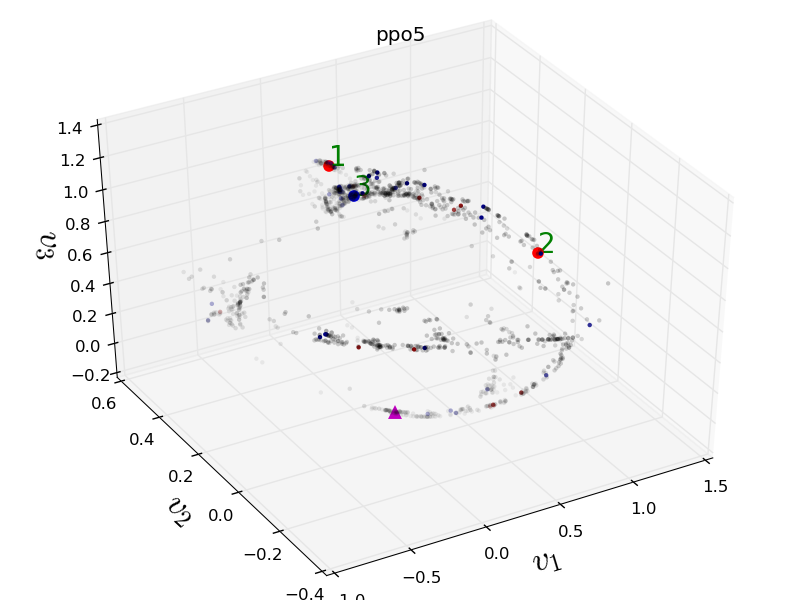
\includegraphics[width = 0.36\textwidth]{ppo5} \\
   \PPO{6} 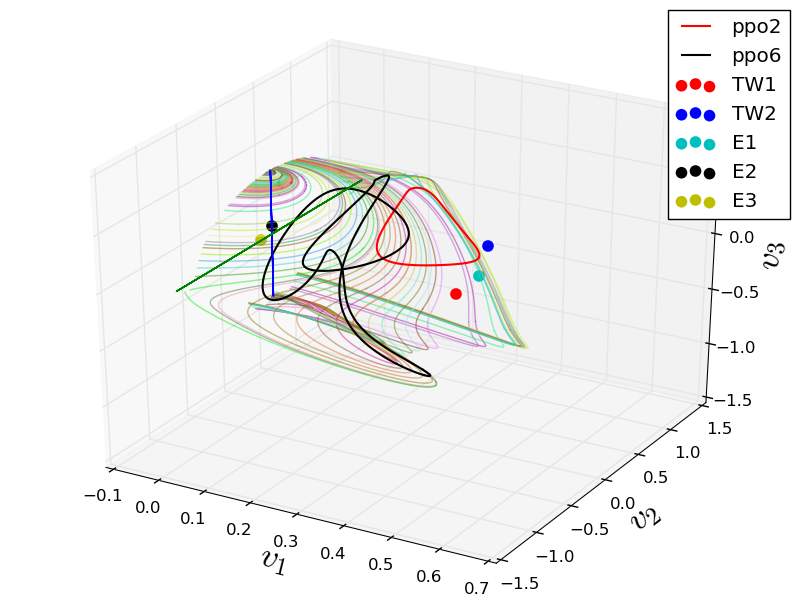
\includegraphics[width = 0.36\textwidth]{ppo6}
   \PPO{8} 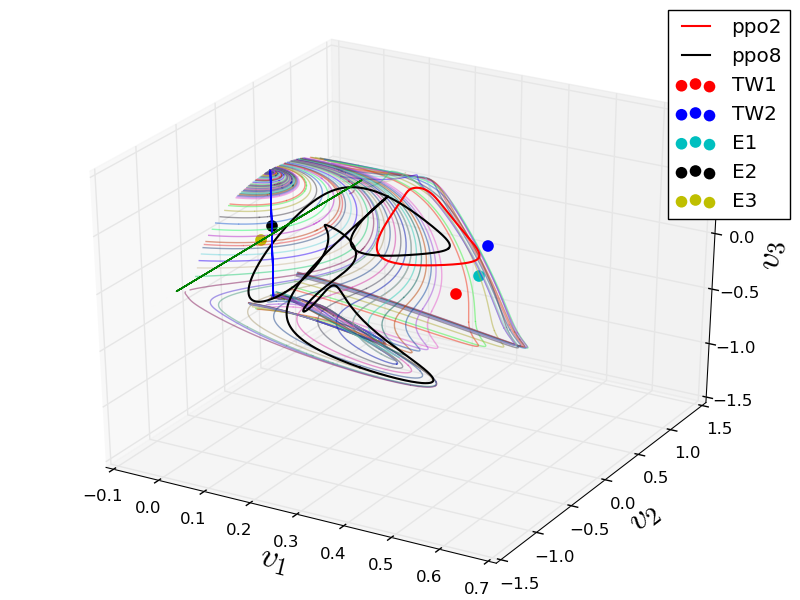
\includegraphics[width = 0.36\textwidth]{ppo8}
\end{center}
   \caption{
In-slice orbits of the fixed points of the fundamental domain border
\PoincSec\ \refeq{eq:ksfundDomain}, with $\alpha_2 = 1$ and all other
$\alpha_k=0$.
         \PPO{2} has no \PoincSec\ fixed point, but (currently) its
         partner \RPO{1} does.
         \PPO{3},
         \PPO{4}.
         \PPO{5} and
         \PPO{6} are partners.
         \PPO{8}.
Projection axes are the imaginary parts of the first 3 Fourier modes
$[v_1, v_2, v_3] = [c_1, c_3, c_2]$, \ie, this is invariant under
reflection in the full \statesp, and in the Xiong's {\fFslice}
\refeq{XDinsliceRefl}.
         }
  \label{fig:ppoFixedPts}
\end{figure}
%%%%%%%%%%%%%%%%%%%%%%%%%%%%%%%%%%%%%%%%%%%%%%%%%%%%%%%%%%%%%%%%%%%%%

\item[2016-06-06 Predrag]
Wonderful - when you look at their \statesp\ plots, they are clearly
sub-segments of longer orbits. For example,
\beq
\PPO{2}+\PPO{4}=\PPO{12}
\ee{pp2-pp4shadowingA}
should be a 2-cycle in the \PoincSec, in the
$\{\PPO{2},\PPO{4},\cdots\}$ alphabet,
and so should be its cousin (so extra letters are needed to distinguish
them):
\beq
\PPO{2}+\PPO{4}=\PPO{14}
\ee{pp2-pp4shadowingB}

\beq
\PPO{2}+\PPO{2}+\PPO{4}=\PPO{30}
\ee{2pp2-pp4shadowing}
should be a 3-cycle.

\beq
\PPO{4}+\PPO{5}=\PPO{42}
\,,\qquad
\PPO{5}+\PPO{6}=\PPO{43}
\ee{pp4-pp5shadowing}
should be a 2-cycles.

Truth be told, \reffig{fig:ppoFixedPts} is a lousy ``alphabet''. But
there are many `glued' longer orbits. A `gluing' example:
\beq
\PPO{2}+\PPO{9}=\PPO{23}
\ee{pp2-pp9shadowing}
so \PPO{23} should be a 3-cycle in the \PoincSec, in the
$\{\PPO{2},\PPO{9},\cdots\}$ alphabet.

\item[2016-06-06 Xiong]
But \PPO{2} does not intersect with \PoincSec\ even
though it shadows \RPO{1}.

\item[2016-06-06 Predrag]
That is not possible. Every \PPO{j} \emph{must} cross the fundamental
domain border \PoincSec. ``It shadows \RPO{1}'' does not matter, why
would it?

\item[2016-06-06 Xiong]
The only \rpo\ that crosses the fundamental domain
border \PoincSec\ is \RPO{1}.

\item[2016-06-06 Predrag]
That is significant. As \RPO{j} / \PPO{j} pairs are exponentially
close almost everywhere, a random \PoincSec\ would cut over them both.
Xiong is saying that for \PPO{j} fixed points, the bifurcation is such
that the sibling \RPO{j} stays within the fundamental domain
(except for the \PPO{2} / \RPO{1} pair, where there is something screwy
going on already).

\item[2016-06-07 Predrag]
The `30' dimensional subspace is a flow-invariant subspace, so for \ppo s
it is essential that $b_2 \neq 0$ at the instant of crossing the section.

\item[2016-06-07 Xiong]
A lot of my observations above are wrong, so I corrected my code.
Let me describes what actually I did.
Let's denote the fundamental domain $\hat{b}_2 > 0$ to be $A$, and the complement
half $\hat{b}_2 < 0$ to be $\bar{A}$. Trajectory crossing fundamental domain
border in way $\bar{A}\to A$ is called $+$, and the other way around $-$.
The direction of the \PoincSec\ is defined as the direction of $+$.

For a PPO, it must cross fundamental domain border for odd number of times in a prime
period, with two possibilities here: $\{+,-,+,-\cdots,+\}$ or
$\{-,+,-,+\cdots,-\}$. Say for the first case, denoting the sequence
of \PoincSec\ points as
$\{p_1, p_2, p_3,\cdots, p_{2n+1}\}$. So the \PoincSec\ sequence
of this PPO is
$\{p_1, p_3, \cdots, p_{2n+1}\}$. The remaining set $\{p_2, p_4, \cdots, p_{2n}\}$
is actually the \PoincSec\ sequence of the reflection orbit
of this PPO, more precisely, the 2nd half orbit if we integrate it for twice prime
period.

\item[2016-06-08 Predrag]
Why do you repeat initial point as the final point? It's like writing
2-cycle \cycle{01} as \cycle{010}. That's wrong $\cycle{010} = \cycle{001}$
is a 3-cycle. Anyway, you count only +'s (or -'s) as \PoincSec\ points,
and the length of \ppo s can be both even and odd...


\item[2016-06-07 Xiong]
A \rpo\ must cross fundamental domain border for even number of times in a prime
period. Say the sequence is $\{p_1, p_2,\cdots,p_{2n}\}$ and the direction is
$\{+,-,+,-\cdots, -\}$. Therefore, sequence  $\{p_1, p_3,\cdots,p_{2n-1}\}$
is the \PoincSec\ points of this \rpo, and sequence
$\{p_2, p_4,\cdots,p_{2n}\}$ is the  \PoincSec\ points of its
reflection twin.

So, in my point of view, though an orbit and its reflection twin are the
same orbit in the fundamental domain, their i\PoincSec\ points are
actually different. Is this logic right or wrong ?

Initially, I observe that \PPO{2} crosses \PoincSec\ in way $-$, so I said it
does not intersect with \PoincSec. Now I think it is wrong. Also, I said
\PPO{3}, \PPO{4}, \PPO{5}, \PPO{6}, \PPO{8} are fixed points, but that is not
correct because their crossing sequences are actually $\{-, +, -\}$. The
reflection twins have 2 \PoincSec\ points.

I updated \reffig{fig:ksfundPoinc}. \RPO{1} has \PoincSec\ points
$\{p_1, p_2\}$ with direction $\{+, -\}$. I choose the second one as the origin
because this one is also very close to the intersection point of \PPO{2}.
Folder \texttt{figs/KSPoincare/} contains the intersection result. The gray dark
background points are the \PoincSec\ points of 100 \rpo s and \ppo s. magenta triangle is
the origin. Red circles are the \PoincSec\ points of the ergodic orbit. Blue circles are
the \PoincSec\ points of its reflection twin. Numbers denote the temporal order.
The order only works for circles with the same color.

\item[2016-07-24 Xiong to Predrag]
I checked that the figures inside folder \texttt{KSPoincare} are correct.
Last time, you were concerned that crossings with opposite directions occur
at every close locations, which indicate my code is wrong. This is actually
not true, because the blue crossings are the \PoincSec\ points of the reflected
orbit. Suppose one orbit crosses the \PoincSec\ as $x_1, x_2, x_3$ with direction
$\{+, -, +\}$, then the
second point is plotted as $\Refl x_2$.

\item[2016-07-26 Predrag]
Isn't the \Zn{2} symmetry quotiented, \ie, aren't $\Refl\ssp$ and $\ssp$
the same point \sspRed\ in the symmetry-reduced \statesp\ \pSRed?

\item[2016-07-26 Xiong]
Yes. reflection is quotiented, but the \PoincSec\ is chosen as the
reflection border $b_2 = 0$. which means intersection point $\ssp$
and its reflection $\Refl\ssp$ are both on \PoincSec\ (still different
points). when the orbit evolve to $\ssp$, then it is reflected to
$\Refl\ssp$ and continues to evolve forward. In this way,
this orbit is kept in the fundamental domain. So
it pieces the \PoincSec\ once, but you get two points.
Direction is needed: $\{+, -, +, \cdots\}$ or $\{-, +, -,\cdots\}$.
This corresponds to considering two orbits together in the slice
(not the fundamental domain).


\item[2016-07-24 Xiong to Predrag]
Some jumps can be classified. For example, the jump from red 1 to
red 2 in \texttt{KSPoincare/rpo/rpo7.png} can be found in
\RPO{8} (blue 3 to blue 4), \RPO{11} (red 2 to red 3), \RPO{19}, \RPO{23},
\RPO{43}, \RPO{45}. The corresponding structure in state space
can be identified by viewing figures in \texttt{KSshadow/rpo/}. I think you know
what structure I mean.
However, some \rpo s do not adhere to this jump rule, like red 1 to red 2 in \RPO{32}.

\item[2016-07-25 Xiong]
In the \HREF{http://www.cns.gatech.edu/~xiong/figs/mixPoincare.html}
{previous visualization}, see \reffig{fig:ksfundPoinc}, Floquet vectors
of one point on \RPO{1} were used to project the \PoincSec\ points, but
there is a dense area in one of the 3 branches. Now, I choose the Floquet
vectors of \RPO{2} to project the \PoincSec\ points. The result is shown
\HREF{http://www.cns.gatech.edu/~xiong/figs/PoPoincare.html}{here}. The
red dots are \PoincSec\ points of the leading 100 \rpo s and \ppo s. Now,
they are nicely separated out in thin, almost 1-dimensional families.

\item[2016-07-26 Predrag to Prophet of Doom]
Indeed, it looks better now:)

I do not remember whether \RPO{2} was embedded into the strange attractor
- is it? According to my eyeballing, it shadows only \RPO{38} and
\RPO{39} (did not check the \ppo s). Of course, \RPO{1} is infrequently
visited, so it was not an obvious choice for a \PoincSec\ template.

Where is the \RPO{2} \PoincSec\ point (or is it 2 points)? Can you mark
it by a fat point, and continue its most unstable Floquet vector into the
(near part of) unstable manifold? Does that capture a part of the strange
attractor generated by an ergodic orbit?

\item[2016-07-26 Xiong to Predrag]
\RPO{2} is embedded in the attractor, may not be visited as frequently
as \RPO{1}. But it has an intersection point in the dense area in the
previous projection, so I chose it as the new origin. I am not saying
that this orbit is any more important than \RPO{1}.
I just feel that 1 dimensional intersection points or several strips of
almost 1 dimensional intersection points are really hard to get.
The chosen \PoincSec\ does not seem optimal.

I will update the figure.

\item[2015-06-01, 2017-03-10 Predrag]
Aston and Laing\rf{AstLai00} {\em Symmetry and chaos in the
complex {Ginzburg-Landau} equation - II. Translational symmetries}
has a clear discussion of spatial period tripling, their sect.~3.2.
They also consider solutions which have reflectional symmetries and are
pre-periodic in $2\pi/3$.
For solutions with spatial period $2\pi/3$ and varying amounts of symmetry
they find that chaotic solutions are
always unstable with respect to perturbations of period $2\pi$.

This might help you classify the solutions of \KS\ at $L=22$, and use that
group theory to construct a natural symbolic dynamics. For example, for the
$N$-disk billiards, that gives the right symbolic dynamics - nothing else is
needed.

\begin{figure}[h]
  \centering
  (a)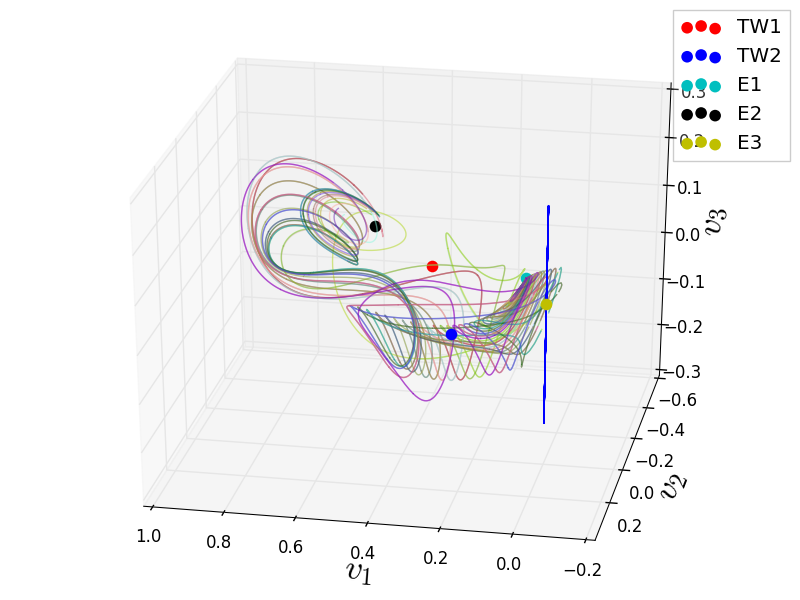
\includegraphics[width=0.45\textwidth]{ksE1Wu2ndModeSlice1}
  (b)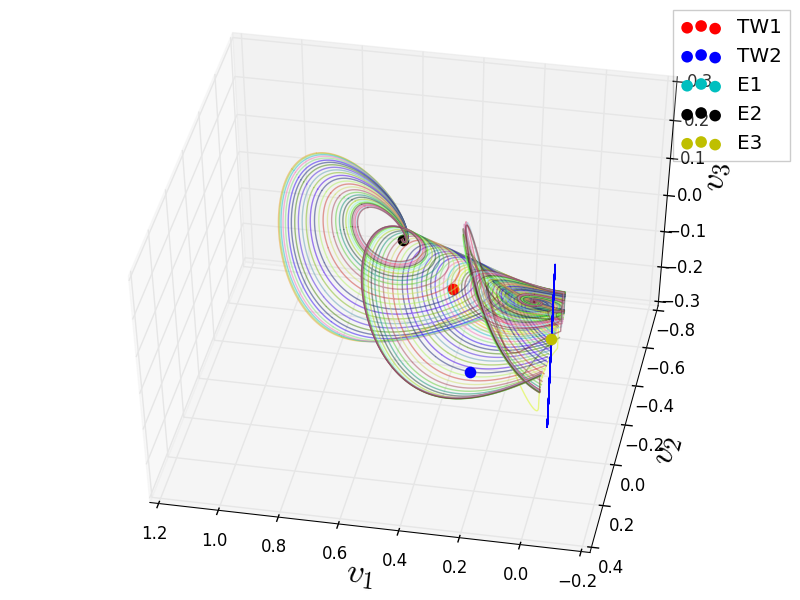
\includegraphics[width=0.45\textwidth]{ksE1Wu2ndModeSlice2}
  \caption{
    \SFslice, fundamental domain \refeq{XDsFslice1} reduction of \On{2}.
    Unstable manifold of \EQV{1}:
    (a) the leading expanding eigenvalus pair, (b) the second expanding pair.
    $[v_1, v_2, v_3] = [\hat{c}_2, \hat{c}_4, \hat{c}_6]$.
  }
  \label{fig:ksE1Wu2nd}
\end{figure}
\begin{figure}[h]
  \centering
  (a)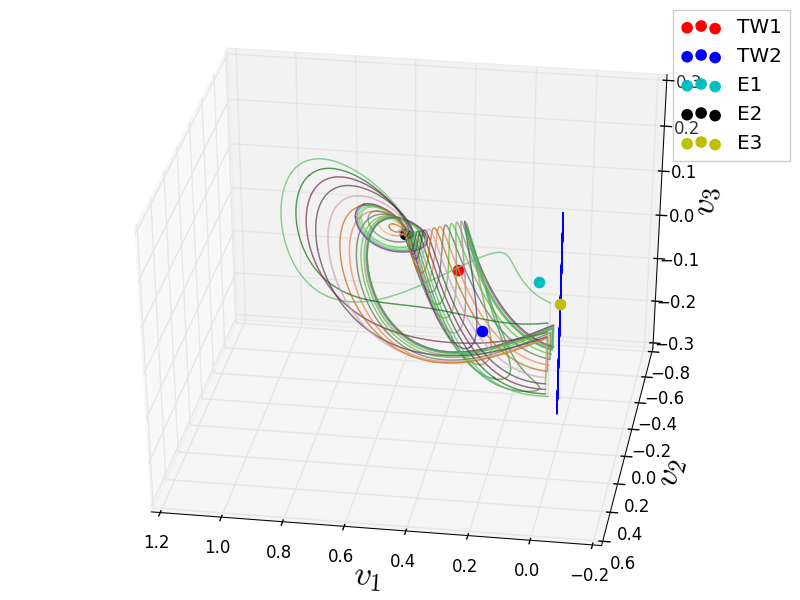
\includegraphics[width=0.45\textwidth]{ksE2Wu2ndModeSlice}
  (b)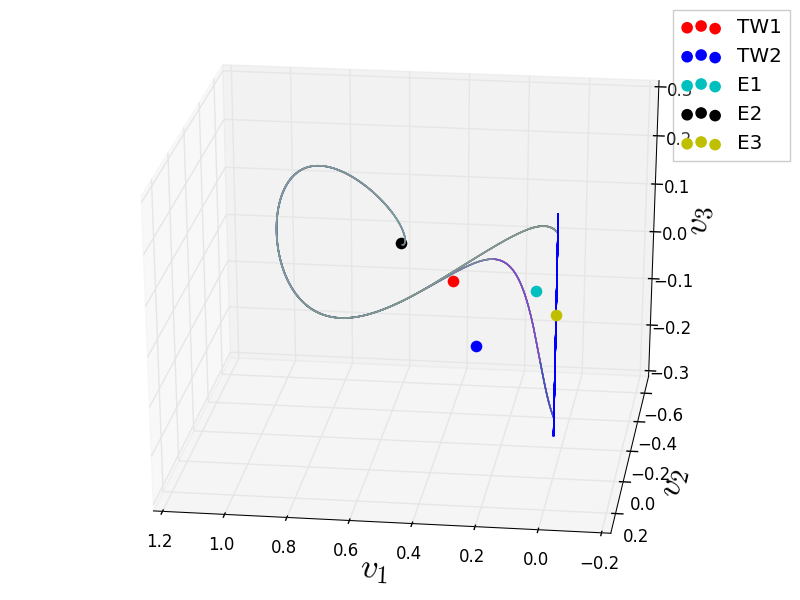
\includegraphics[width=0.45\textwidth]{ksE3Wu2ndModeSlice}
  \caption{
    \SFslice, fundamental domain \refeq{XDsFslice1} reduction of \On{2}.
    Unstable manifolds of \EQV{2} (contained in $\bbU^+$) and \EQV{3}.
    }
  \label{fig:ksWuE2E32nd}
\end{figure}


\item[2017-03-11 Xiong]
I am returning to the {\sFslice}. The reason is that I really want to
figure out what orbits are doing when they are close to \EQV{2}.
In the {\fFslice}, an orbit just traces out circles when
it gets close to \EQV{2}, which is in the slice border.


 {\bf \SFslice} reduction of \On{2} is defined by rotation into
In contrast to \refeq{XDsFslice} and \reffig{fig:ksE2Wu},
which use polynomials to reduce reflection, now  I use the
3rd Fourier mode to define a fundamental domain.
\bea
b_2 &=& 0 \,\quad c_2 > 0,
    \continue
\hat{b}_3 &>& 0\quad \text{and} \quad \hat{c}_3 > 0
\,,
\label{XDsFslice1}
\eea
where $\hat{a}_k = b_k+ic_k$. With this choice the reflection
\refeq{XDsFsliceRefl} does not change its rule  after reducing $\SOn{2}$.

\refFig{fig:ksE1Wu2nd} and \reffig{fig:ksWuE2E32nd} show the
unstable manifold of the three equilibria. Here, again I not
using projection to the eigen-directions. The first
reason is that I am lazy. Projection requires a few more lines
of code. The second reason is that I am concerned about such
an projection. The obvious choice of projection bases is the
eigenvectors of \EQV{2}, but its eigenvectors are in the
antisymmetric subspace. So after projection, half number of
degrees of freedom vanishes. I choose Fourier projection bases
$[\hat{c}_2, \hat{c}_4, \hat{c}_6]$ because they are invariant
under reflection making figures more pleasing.

\EQV{3} is in the slice border.
The blue vertical lines in these two figures are the group orbit
of \EQV{3}. It is interesting that the unstable manifold of \EQV{3}
comes out of the slice border from two different locations and then
merges at some point. These two heteroclinic orbits are not related
to each other by some symmetry. In \rf{SCD07},
the unstable manifold of \EQV{3} has 3 branches. In the 2nd mode slice,
there are two branches.

I also plotted 50 \RPO{}s in the \texttt{figs/KSshadow/rpo2ndModeSlice}.
All these figures are similar to the previous result using invariant
polynomials in \reffig{fig:ksE2Wu}. At least in this 3d projector, the
attractor seems thin. Almost every \RPO{} will get close to the slice
boarder once. Still, it is hard to tell what the orbit is doing when
it gets close to \EQV{3} except from plotting circles.
My plan is to use two Poincare sections. One is at \EQV{2} and the other
is at \EQV{3}, but \EQV{3} is in the slice border which leads me to
give up.

How about using power figure to get rid of \On{2}? We may get
some false positive symbolic dynamics, but afterwards we can
check the result in the slice.

\item[Xiong 2017-03-18]
I have had a look at the 3rd mode slice. \refFig{fig:tFslice} shows the
result. \EQV{2} is in the slice boarder. The 3rd mode slice is not as
interesting as the {\sFslice}e.

\begin{figure}[h]
  \centering
  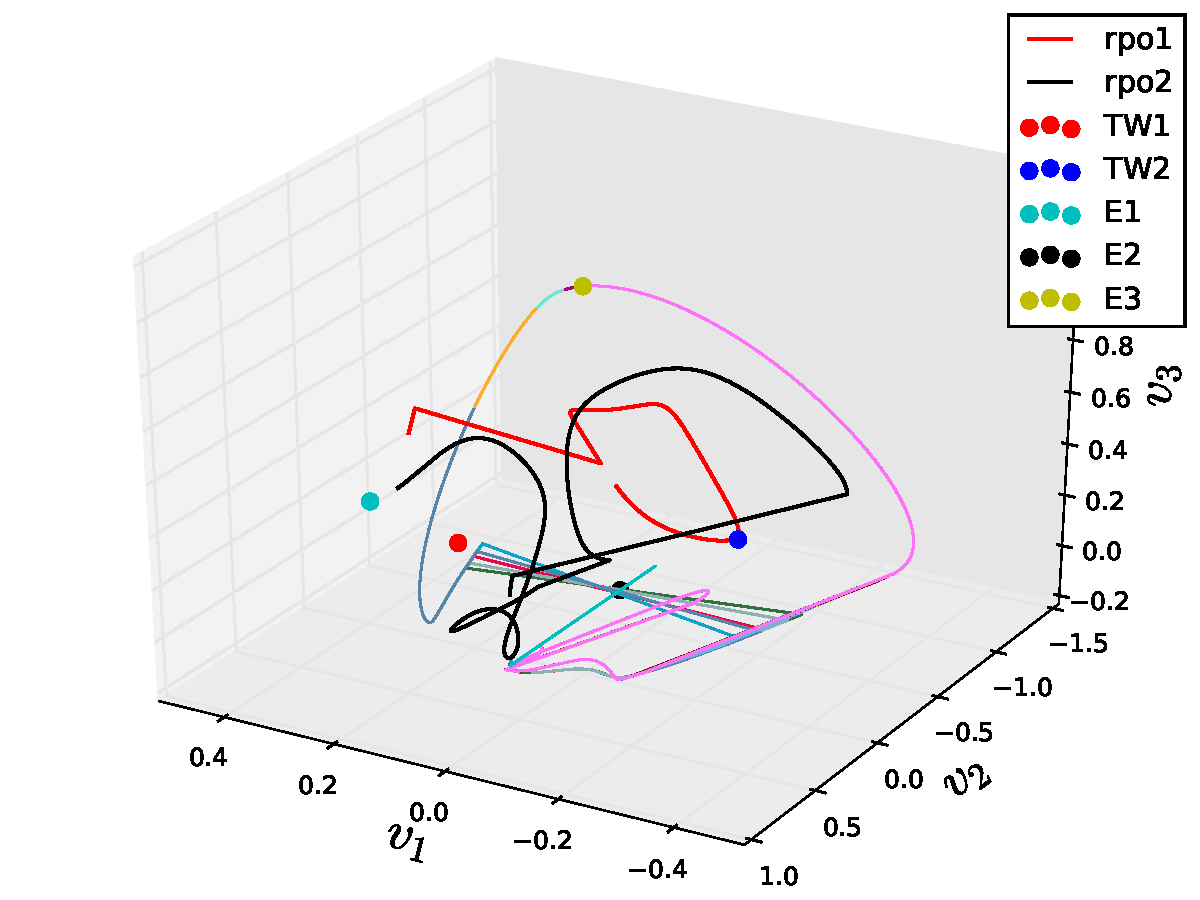
\includegraphics[width=0.7\textwidth]{ks3rdSliceExam}
  \caption{
    3rd mode slice. The yellow and pink curves are the unstable manifold
    of \EQV{3}. The green straight line is the group orbit of \EQV{2}.
  }
  \label{fig:tFslice}
\end{figure}

\item[2017-03-19 Predrag]
I agree with you - at $L=22$ the \EQV{2} unstable mode is the dominant
structure in the \statesp, 3rd mode slice is not as interesting. I still
prefer the {\fFslice}, because I worry about what to pick for larger  $L$.

\item[2009-04-07, 2017-03-15 Predrag]
A possible way forward is inspired by 3-disk billiard's symbolic
dynamics. That one is generated by the sequence of \Dn{3} generators
(``0'' for 1/3 shift, ``1'' for reflection), and a pair of \PoincSec s,
one for each symmetry axis border of the fundamental domain.
Due to the simplicity of the problem, that happens to result in the full
\statesp\ partition, there are no further subpartitions that could have
arisen due to nonlinear effects. That is in contrast to the standard map
- global winding number gives a coarse covering symbolic dynamics, but
then individual tori add further refinements.

The idea is this: After \SOn{2} symmetry reduction, all its $C_n$
discrete symmetry subgroups survive as exact discrete symmetries of
dynamics; an example of such symmetry is $C_2$ symmetry utilized in
ChaosBook to define a fundamental domain (a half-space) for the Lorenz
system. For \KS\ we have utilized the $C_2$ subgroup in \refref{SCD07} to
construct \Dn{2} invariant subspaces (see \refeq{ek_defn1}; this whole
project started with this proposal elaborate here, see
\refsect{sec:KSeSymm}), but have not done much with \Dn{3}.

For \KS, so far we have only utilized $\Refl$ invariance to construct our
first \PoincSec. I propose we next use the \Dn{2} fundamental domain to
construct the next \PoincSec; that restricts all $2k$ Fourier multiples
to a half-space, and introduces one new symbol (1/2 shift needed to pull
the point into the fundamental domain). Then we add the \Dn{3} \PoincSec;
that restricts all $3k$ Fourier multiples to a third-space, and
introduces two new symbols (1/3 or 2/3 shift) needed to pull the point
into the fundamental domain (which is $1/(2*2*3)=1/12$ of the full
\statesp). While in principle one could continue to \Dn{4} \PoincSec,
etc, nothing is gained, as for $L=22$ there are no \reqva\ or
pre-periodic orbits with higher discrete symmetries.

So itinerary would be would be an admissible sequence of letters from
the alphabet consisting of operations that return the \statesp\ to
the fundamental domain, whenever it crosses any of its borders:
\begin{itemize}
  \item a reflection (for the current anti-symmetric subspace section)
  \item 1/2 rotation (return to the the \Dn{2} fundamental domain border / \PoincSec)
  \item 1/3 and 2/3 (or -1/2) rotations
  (return to the the \Dn{3} fundamental domain border / \PoincSec)
\end{itemize}

That is guaranteed to give us a rough covering symbolic dynamics for
$L=22$. Whether it gives us full subshift (1-1 mapping between orbits and
itineraries) remains to be seen.

First, some text copied from \refref{SCD07}:

Any rational shift $ \Shift_{1/m}u(x)=u(x+L/m)$ generates a discrete
cyclic subgroup $C_m$ of $O(2)$, which is also a symmetry of KS
system. Reflection together with $C_m$ generates another
symmetry of KS system, the dihedral subgroup $\Dn{m}$ of $O(2)$.
The only non-zero Fourier components of a solution invariant
under $C_m$ are $a_{jm} \neq 0$, $j =1,2,\cdots$, while for a
solution invariant under $\Dn{m}$ we also have the condition
$\Re a_j=0$ for all $j$.
For example, the 1/2-cell translations \beq
    \Shift_{1/2}\, u(x)=u(x+L/2)
\ee{KSshift}
and reflections generate $O(2)$
subgroup $\Dn{2} = \{1, \Refl,\Shift,\Shift\Refl\}$,
which
reduces the \statesp\ into four irreducible subspaces
(for brevity, here $\Shift = \Shift_{1/2}$):
\begin{align}
 & \qquad\qquad\qquad\qquad\qquad
              ~~~ \Shift ~~ \Refl  ~\;  \Shift\Refl
    \nnu\\
P^{(1)} &= \frac{1}{4} (1 + \Shift + \Refl + \Shift\Refl)
           ~~~~  S  ~~  S   ~~   S
    \nnu\\
P^{(2)} &= \frac{1}{4} (1 + \Shift - \Refl - \Shift\Refl)
            ~~~~  S  ~~  A   ~~   A
    \nnu\\
P^{(3)} &= \frac{1}{4} (1 - \Shift + \Refl - \Shift\Refl)
           ~~~~  A  ~~  S   ~~   A
     \label{ek_defn1}\\
P^{(4)} &= \frac{1}{4} (1 - \Shift - \Refl + \Shift\Refl)
          ~~~~  A  ~~  A   ~~   S
\,.
    \nnu
\end{align}
$P^{(j)}$ is the projection operator onto
$u^{(j)}$ irreducible subspace, and the last 3 columns
refer to the symmetry (or antisymmetry) of
$u^{(j)}$ functions under reflection and
1/2-cell shift.
By the same argument that identified \refeq{KSU+} as
the invariant subspace of KS, here the KS flow
stays within the
 $\bbU^S =  \bbU^{(1)}+ \bbU^{(2)}$
irreducible $\Dn{1}$ subspace of
$u$ profiles symmetric under 1/2-cell shifts.

While in general the bilinear term $(u^2)_x$  mixes the
irreducible subspaces of $\Dn{m}$, for $\Dn{2}$ there are
four subspaces invariant under the flow\rf{KNSks90}:
\begin{description}
 \item[$\{0\}$:~~~~~~] the $u(x)=0$ {\eqv}
 \item[$\bbU^+ = \bbU^{(1)}+ \bbU^{(3)} $:]
    the reflection $\Dn{1}$ irreducible space of antisymmetric $u(x)$
 \item[$\bbU^S =  \bbU^{(1)}+ \bbU^{(2)}$:]
    the shift $\Dn{1}$ irreducible space of $L/2$ shift symmetric  $u(x)$
 \item[$\bbU^{(1)}$:~~~~~]
    the $\Dn{2}$ irreducible  space of $u(x)$ invariant under $x\mapsto L/2-x,\ u\mapsto -u$.
\end{description}
With the continuous
translational symmetry eliminated within each subspace, there are no
\reqva\ and \rpo s, and one
can focus on the \eqva\ and \po s only, as was done
for $\bbU^+$ in \refrefs{Christiansen97,LanThesis,lanCvit07}.
In the Fourier
representation, the
$u \in \bbU^+$
antisymmetry amounts to having purely imaginary
coefficients, since $a_{-k}= a^\ast_k = -a_k$.
The 1/2 cell-size shift $\Shift_{1/2}$
generated 2-element discrete subgroup
$\{1,\Shift_{1/2}\}$ is
of particular interest
because in the $\bbU^+$ subspace the translational invariance of the full system reduces to
invariance under discrete translation \refeq{KSshift} by half a
spatial period $L/2$.

Due to the KS equation invariance under
the dihedral $D_n$ and cyclic $C_n$ subgroups, the following
types of \po s are possible:

{\bf (a)} The \po\ lies
within a subspace pointwise invariant under the action of
$D_n$ or $C_n$. For instance, for $D_1$ this is the
$\bbU^+$ antisymmetric subspace, $-u_p(-x) = u_p(x)$, and
$u(x,\period{p}) = u(x,0) = u_p(x)$. The periodic orbits
found in \refrefs{Christiansen97,lanCvit07} are
all in $\bbU^+$, as the dynamics is restricted to
antisymmetric subspace. For $L=22$ the dynamics in $\bbU^+$
is dominated by attracting (within the subspace)
heteroclinic connections and thus we have no periodic orbits
of this type, or in any other of the $D_n$--invariant
subspaces, see \refref{SCD07}. %\refsect{sec:L22}.

{\bf (b)} The \po\ satisfies
\beq
	 u(x,t+\period{p})=\gamma u(x,t)\,,
	\label{eq:POspattemp}
\eeq
for some group element $\gamma\in O(2)$ such that
$\gamma^m=e$ for some integer $m$ so that the orbit repeats
after time $m \period{p}$ (see
\refref{golubitsky2002sp} for a general discussion of
conditions on the symmetry of \po s).
If an orbit is of reflection type, % \refeq{KSpos},
$\Refl\Shift_{\shift/L} u(x,\period{p}) =
-u(-x-\shift,\period{p}) = u(x,0)$, then it is pre-periodic
to a \po\ with period $2\period{p}$. Indeed, since
$(\Refl\Shift_{\shift/L})^2 = \Refl^2 = 1$, and the KS
solutions are time translation invariant, it follows % from \refeq{KSpos}
that
\[
  u(x,2\period{p}) = \Refl\Shift_{\shift/L} u(x,\period{p}) =
  (\Refl\Shift_{\shift/L})^2 u(x,0) = u(x,0)\;.
\]
Thus any shift acquired during time $0$ to
$\period{p}$ is compensated by the opposite shift during
evolution from $\period{p}$ to $2 \period{p}$.
All periodic orbits we have found for $L=22$ are of type
\refeq{eq:POspattemp} with $\gamma=R$. Pre-periodic orbits
with $\gamma\in C_n$ have been found by Brown and
Kevrekidis\rf{BrKevr96} for KS system sizes larger than ours,
but we have not found any for $L=22$.
Pre-periodic orbits are a hallmark of any dynamical system
with a discrete symmetry, where they have a natural
interpretation as \po s in the fundamental
domain\rf{CvitaEckardt,DasBuch}.

\item[Xiong 2017-03-18]
\refFig{fig:ksFund}
shows the fundamental domains when we using different slices.
What does the $1/12$ domain refer to? one half of the panel (c)
in \reffig{fig:ksFund}?
%%%%%%%%%%%%%%%%%%%%%%%%%%%%%%%%%%%%%%%%%%%%%%%%%%%%%%%%%%%%%%%%
\begin{figure}[h]
  \centering
  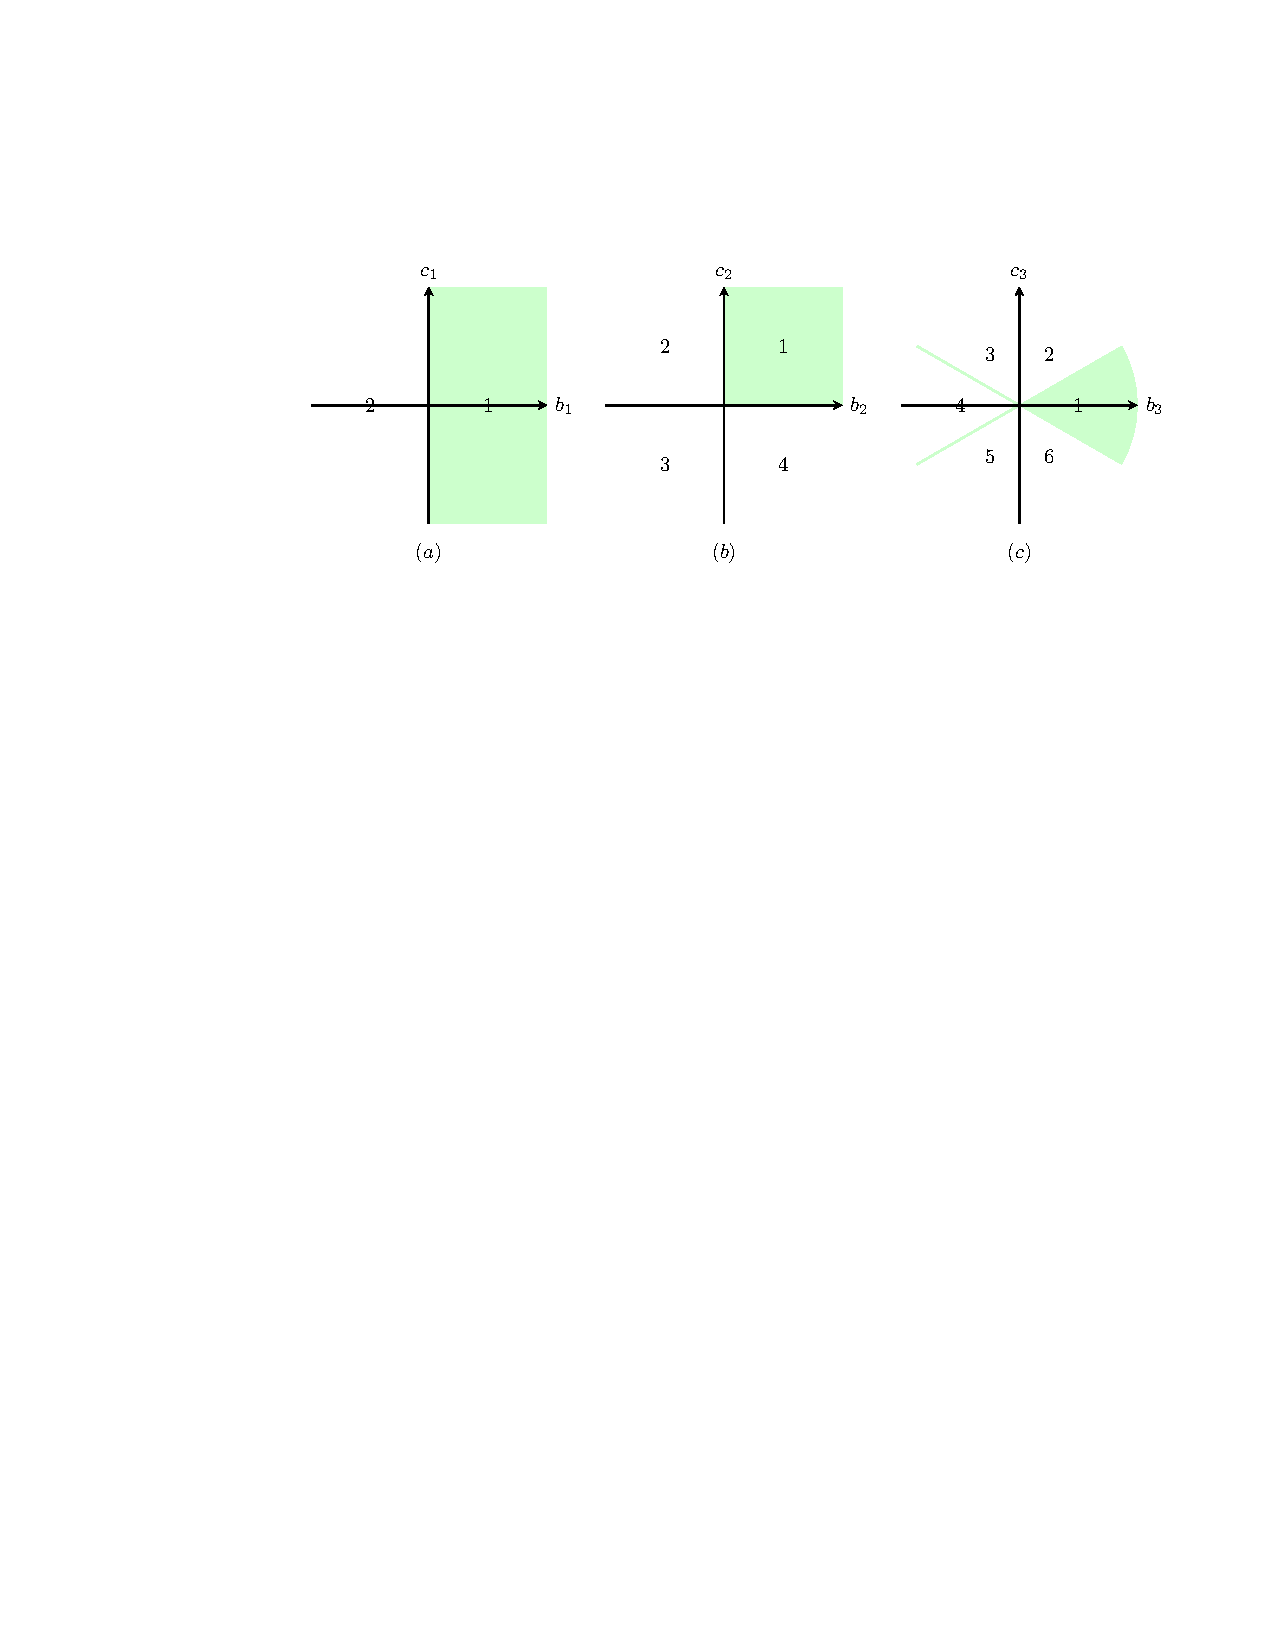
\includegraphics[width=0.95\textwidth]{ksFund}
  \\
  (d) 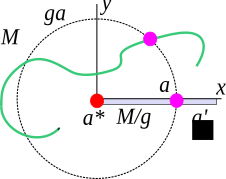
\includegraphics[width=0.32\textwidth]{FourierSlice}
  \caption{
    Fundamental domain using {\fFslice}, followed by (a) $\Dn{1}$
    reduction under $\Refl$. This is then followed by defining (b)
    $\Zn{2}$ fundamental domain; then (c) $\Zn{3}$ fundamental domain.
    Each projection is on the $(b_i,c_i)$ complex plane - all
    other Fourier modes are projected into the origin.
    (d) \FFslice\ reduces a whole dimension, so presumably the correct
    version of (a) is a half-line, not half-plane.
  }
  \label{fig:ksFund}
\end{figure}
%%%%%%%%%%%%%%%%%%%%%%%%%%%%%%%%%%%%%%%%%%%%%%%%%%%%%%%%%%%%%%%%
\item[2017-03-19 Predrag]
In case of the $\Zn{n} \in \SOn{2}$ symmetry, the choice of the rightmost
border of a fundamental domain is conventional, all orientations are
equally good. I think it would be more consistent to define all domains
in \reffig{fig:ksFund} by setting the angle of the rightmost border to
zero, either with respect to the $x$-axis (the conventional choice), or
with respect to the $y$-axis
(Xiong's choice, justified by invariance under the reflection $\Refl$).
\refFig{fig:ksFund}\,(c) should be 1/3 of the pizza, not 1/6.

\item[Xiong 2017-03-18]
I cannot get the idea of using \Dn{2} fundamental domain after
constructing a \PoincSec\ by using reflection $\Refl$, and then
constructing another \PoincSec\ by \Dn{3}.
Still I have no idea why we need to
consider the border of a fundamental domain. Like panel (b),
the boarder consist of positive $b_i$ and positive $c_i$ axes,
but if we rotate the fundamental domain (green region), then
the border changes.


\item[2017-03-19 Predrag]
My thinking is all motivated by the 3-disk pinball of ChaosBook, like this.
For a billiard, boundary of the billiard defines the natural \PoincSec.
However, for a smooth flow, that does not exist. If the smooth potential
has \Dn{3} symmetry (think 3 hills, rather that 3 infinite height cylinders),
the two
\PoincSec s placed on the symmetry axes borders of the fundamental
domain (1/6th of the pizza) are natural sections, both for billiards and for
smooth flows. Those are the sections Tingnan and I use in
\HREF{https://github.com/cvitanov/reducesymm/} {gitHub.com/cvitanov/reducesymm}.

Whenever you leave the fundamental domain, there is a group operation for
that border that puts you back in the domain. That is why you want to use
borders of the fundamental domain.

First (I think - not sure what is the best order in which to reduce) we
slice $\SOn{2}$, decreasing the \emph{dimension} of \statesp\ by 1.
$\Dn{1}$ reduction, under $\Refl$, makes the fundamental domain
$\PoincS_1 \in \bbU^+$ a
1/2-space; from now on all \PoincSec s will be in its border,
$\PoincS_j \subset \bbU^+$.
    \PCedit{(My \reffig{fig:ksFund}\,(a) caption is surely nonsense,
            see \reffig{fig:ksFund}\,(d). Also I presume all other
            $b_j=0$ as well, so half of the axes labels are wrong?)}
$\Zn{2}$ is described above - fundamental domain is now 1/4-space. For
$\Zn{2}$ one border (0 angle) coincides with the $\PoincS_1$ you have just
constructed, and the other border is the new
$\PoincS_2 \in \bbU^+$, $\Zn{2}$-specific, that
rotates everyone by $2\pi/2$ whenever $\cos 2\phi$ exits the fundamental
domain.
For $\Zn{3}$ the other border is the new $\PoincS_3 \in \bbU^+$,
$\Zn{3}$-specific, that rotates everyone by $2\pi/3$ whenever $\cos
3\phi$ exits the fundamental domain.
    \PCedit{(Hope that this rotation does not conflic with the \fFslice?
    Also, this rotation might move the point out of the $\Zn{2}$
    fundamental domain - in that case one needs to rotate that back, then
    recheck where one is in the $\Zn{2}$ fundamental domain? Yech...)}
Fundamental domain is now 1/12-space. If it pleases the eye, one can plot
it as one continuous domain by appropriate angle-doubling (as for the
Lorenz fundamental domain) and angle tripling; but I see no point of
doing we, we only care about the \PoincSec s, not about the continuous
time trajectory. The reflections remain discontinuous, as in your figures
above.

You track a trajectory $\sspRed(\zeit)$ in the \On{2}-{\reducedsp}. At
the $k$th crossing of a section, $\sspRed_k\in\PoincS_j$, one records the
discrete group element ${\LieEl}_k$ that reflects or rotates the
trajectory back into the fundamental domain, and then restarts the
trajectory there.

Does this make sense?

\item[2017-03-19 Xiong]

  \emph{
    Hope that this rotation does not conflic with the \fFslice?
    Also, this rotation might move the point out of the $\Zn{2}$
    fundamental domain - in that case one needs to rotate that back, then
    recheck where one is in the $\Zn{2}$ fundamental domain? Yech...
  }


  This is the exact part that confused me.
  We can use a Fourier mode to define a slice. Then we use another
  Fourier mode to define a fundamental domain, which is $1/2$ or
  $1/4$ or $1/6$  of the slice by using the 1st or 2nd or 3rd mode.
  Because in the slice, the symmetry becomes \Refl\,, \Dn{2} and
  \Dn{3} respectively.
  How could we defined  two compatible fundamental domains by
  two different Fourier modes? If we rotate in-slice states into
  one fundamental domain, then it can get out of the other fundamental
  domain, or even out of the slice.

  In the slice, \Refl\ and \Zn{2} respectively
  take form
  \[
    \Refl = [-\,, +\,,-\,, +\,,\cdots, -\,, +\,] \,,\quad
    C^{1/2} = [-\,, -\,,+\,, +\,,\cdots, -\,, -\,]
  \]
  The in-slice state is $[\hat{b}_1, \hat{c}_1, \cdots]$.
  A positive sign means that the corresponding component keeps unchanged.
  A minus sign means that the sign flips.
  If we use the 1st mode slice, then $\hat{b}_1 = 0, \hat{c}_1 > 0$.
  We can only
  define a fundamental domain by \Refl\ because,
  given an in-slice state $\sspRed$,
  the $\hat{c}_1$ component of $\Refl \sspRed$ keeps unchanged.
  We cannot define a
  fundamental domain by
  \Zn{2} because $C^{1/2}$ will rotate the state out of slice.

\item[2017-03-20 Predrag]
Maybe I'm making this too complicated by insisting that one rotates into
the fundamental domain... Can we just put stationary \PoincSec s, keep
track of crossing them? For example, in 3-disk billiard $\Dn{3}$
symmetry, there are 6 \PoincSec s in the full \statesp, a 'short' and
'indefinite' halves of each symmetry axis. It would be the same $\Zn{3}$
for \KS; we put \PoincSec\ at angles 0, 1/3 and 2/3? Then nothing has to
be rotated, but in plotting the sections, we plot all three on top of
each other.

\item[2017-03-21 Burak]
I might be missing a point but I don't think the analogy between 3-disk
problem and \KS\ really works. When we use \fFslice\ to reduce \SOn{2} ,
within the \slice , the only remaining symmetry is the reflection.
So we don't really have $\Dn{2}$ or $\Dn{3}$ symmetries in the \fFslice .
Subspaces corresponding to wavenumbers that are multiples of $2$ and $3$
are in the \sliceBord , so in these subspaces,
we don't only have $\Dn{2}$ and $\Dn{3}$ but in fact we have full
$\On{2}$, respectively. Although, we can count number of crossing between
regions highlighted in \reffig{fig:ksFund}(b and c) in \fFslice , I don't
quite understand the motivation.

\NBBpost{2017-03-21}{
A proposal: run the same trajectory
simultaneously on \fFslice, \sFslice, and 3rd Fourier mode
slice, and record the instants and group elements where it crosses \PoincSec
s defined within borders of their \Zn{j} fundamental domains. This might
associate a good symbolic string to a given trajectory. We are very uncertain
about the likelihood of this method producing a good covering dynamics. Like,
do we ever cross the 3rd mode \PoincSec s? When \EQV{3} is so far from the
attractor?
}

\item[2017-04-14 Xiong]
I decreased the domain size a little bit and continue the shortest 5
relative/pre-\po s. \PPO{1}, \PPO{2} and \RPO{2} exist even when
the domain size $L$ is as small as $21.2$. But others are not so lucky.
For example, \RPO{3},\RPO{4},\RPO{5} does not converge even for 
$L = 21.9$. Also, we know that for $L=22$, \PPO{2} shadows \RPO{1}.
But \PPO{2} exists for $L\in[21.2, 22]$,
while \RPO{1} exits for $L\in[21.45, 22]$. The shadowing 
does not continue once $L$ is less than 21.45.

\refTab{tab:ks_stab_rpo2} shows the Floquet exponents of \RPO{2}.
The transition from $L=21.85$ to $L=21.8$ is wired. The only one 
pair of unstable directions become real.
\begin{table}[h]
  \centering
  \begin{tabular}{c|ccccc}
    $L$       &  21.95  &  21.90   & 21.85   & 21.80  & 21.75  \\
    \hline
    $T_p$     & 33.247  &  33.854  & 34.570  & 35.239 & 35.811 \\
    $\mu$     &  0.017  &  0.0138  & 0.00998 & 0.0323 & 0.0437 \\
    $\theta$  &  1.469  &  1.728   & 2.358   &  $\pi$ &  $\pi$
  \end{tabular}
  \caption{
    The leading Floquet exponent of \RPO{2} for different domain size.
    Floquet multiplier is given 
    as $\Lambda = \exp(T_p\mu \pm i\theta)$ for complex ones.
    $\theta = 0, \pi$ for real ones.
  }
  \label{tab:ks_stab_rpo2}
\end{table}


\end{description}
